\documentclass[10pt, aspectratio=169]{beamer}

% Configuration {{{
\usepackage[utf8]{inputenc}
\usepackage[T2A]{fontenc} % T1 for English
\usepackage[english, russian]{babel}

\usepackage{mathtools}
\usepackage{graphicx}
\usepackage{tikz}
\usepackage[multidot]{grffile}
\usepackage[labelsep=period]{caption}
\usepackage{multirow}

\setbeamertemplate{caption}[numbered]
\setbeamertemplate{navigation symbols}{}
\usefonttheme[onlymath]{serif}
\usepackage{DejaVuSansCondensed} % helvet for English
\usetheme{Madrid}

\linespread{1.2}
% }}}

% Definitions {{{
\def\pip{\pi^+}
\def\pim{\pi^-}
\def\piz{\pi^0}
\def\rhop{\rho^+}
\def\rhom{\rho^-}
%}}}

% Title and other {{{
\title[Study of $e^+e^- \rightarrow 2\pi3\pi^0$ and $2\pi2\pi^0\eta$]{
  Study of the reactions
  $e^+e^- \rightarrow \pi^+\pi^-\pi^0\pi^0\pi^0$
  and $\pi^+\pi^-\pi^0\pi^0\eta$ at center-of-mass energies
  from threshold to 4.35~GeV using initial-state radiation
  by BaBar Collaboration
  -- contents analysis
}
\author[Kerim Guseynov]{
  Kerim Guseynov \\[2ex] Based on \texttt{arXiv:1810.1196}
}
\institute[MSU]{
  Faculty of Physics \\ Moscow State University
}
\date{Nov 25, 2022}
%}}}

\begin{document}

\frame[plain]{\titlepage}

\begin{frame}[label=intro]%{{{
  \frametitle{Introduction}

  \large
  \begin{itemize}
    \item Initial-state radiation (ISR) includes events like
      $ee\to X \gamma$, where $\gamma$ carries a huge momentum and comes 
      from the initial $ee$ before $ee \to X$.
    \item ISR gives access to a wide range of effective center-of-mass 
      energies below the full $ee$ c.m.~energy.
    \item Gives access to low-energy cross-sections at high luminosity 
      $B$-factories.
      \\ Especially interesting for the muon $g-2$ studies --- the cross 
      sections are required for the Standard Model calculations.
    \item In addition, IRS further facilitates resonance spectroscopy.
  \end{itemize}
\end{frame}%}}}

\begin{frame}[label=babar]%{{{
  \frametitle{{BaBar} detector and data sample}
  \centering
  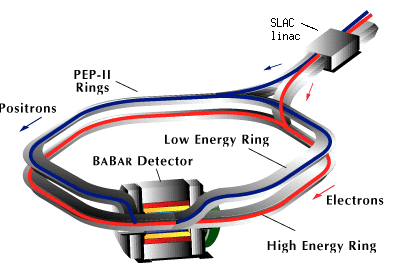
\includegraphics[width=.4\textwidth]{figures/002/babar-scheme}
  \hfill
  
\includegraphics[width=.56\textwidth]{figures/002/upsilon}

  \vskip 2ex
  $\int \mathrm{d} \mathcal{L} = 468.6$ fb$^{-1}$
  \vskip 1ex
  Effective $E_\text{c.m.} < 4.35$ GeV to suppress $\Upsilon(4S)$ 
  background.

  \vskip 2ex \hfill\null
  \textbullet{} Vertex tracker \hfill\hfill
  \textbullet{} Drift chamber \hfill\hfill
  \textbullet{} Cherenkov detector \hfill\null

  % The measurements presented in this paper are based on 383 × 10 
  % 6 Υ (4S) → BB decays recorded with the B A B AR detector [18] at the 
  % PEP-II e+ e− asymmetric-energy B Factory at the Stanford Linear 
  % Accelerator Center. At the interaction point, 9- GeV electrons 
  % collide with 3.1- GeV positrons at the Υ (4S) resonance with 
  % a center-of- mass energy of 10.58 GeV/c2 .
  % Charged particle trajectories are measured by a five- layer silicon 
  % vertex tracker (SVT) and a 40-layer drift chamber (DCH) immersed in 
  % a 1.5-T axial magnetic field. Charged particle identification is 
  % provided by ionization energy (dE/dx) measurements in the SVT and 
  % DCH along with Cherenkov radiation detection by an internally 
  % reflecting ring-imaging detector (DRC).
\end{frame}%}}}

\begin{frame}[label=simulation]%{{{
  \frametitle{Monte Carlo simulation}
  \Large

  \begin{itemize}
    \item $ee \to \pip\pim3\piz\gamma$
      \begin{itemize}
        \item $\omega(782)\piz\piz$
          \\ $\omega(782) \to \pip\pim\piz$
          \\ $\piz\piz$ produced both directly and via $f_0(980)$
        \item $\eta\rho(770)$
          \\ $\eta\to$ all measured modes
      \end{itemize}

    \item $ee \to \pip\pim2\piz\eta\gamma$
      \begin{itemize}
        \item Phase-space model
        \item $\omega\piz\eta$
      \end{itemize}

    \item Large background samples of both ISR and non-ISR prosesses.
  \end{itemize}
\end{frame}%}}}

\begin{frame}[label=selection]%{{{
  \frametitle{Event selection}
  \large

  \begin{itemize}
    \item Two pion tracks (from interaction region) and at least 
      7~photons.
    \item The largest-energy $\gamma$ is considered the ISR one.
    \item The other 6 are grouped in two pairs around $m_\pi$ and two 
      independent ones: both $\piz$ and $\eta$.
    \item Each event is fit with signal hypothesis 
      $ee\to\pip\pim3\piz\gamma$ and bkg hypothesis 
      $ee\to\pip\pim2\piz\gamma$ (much larger cross-section).
      \\ $\chi^2$ from the fits are used later for bkg subtraction.
  \end{itemize}
\end{frame}%}}}

\begin{frame}[label=3pi-selection]%{{{
  \frametitle{$\pip\pim3\piz$: event selection}
  \centering

  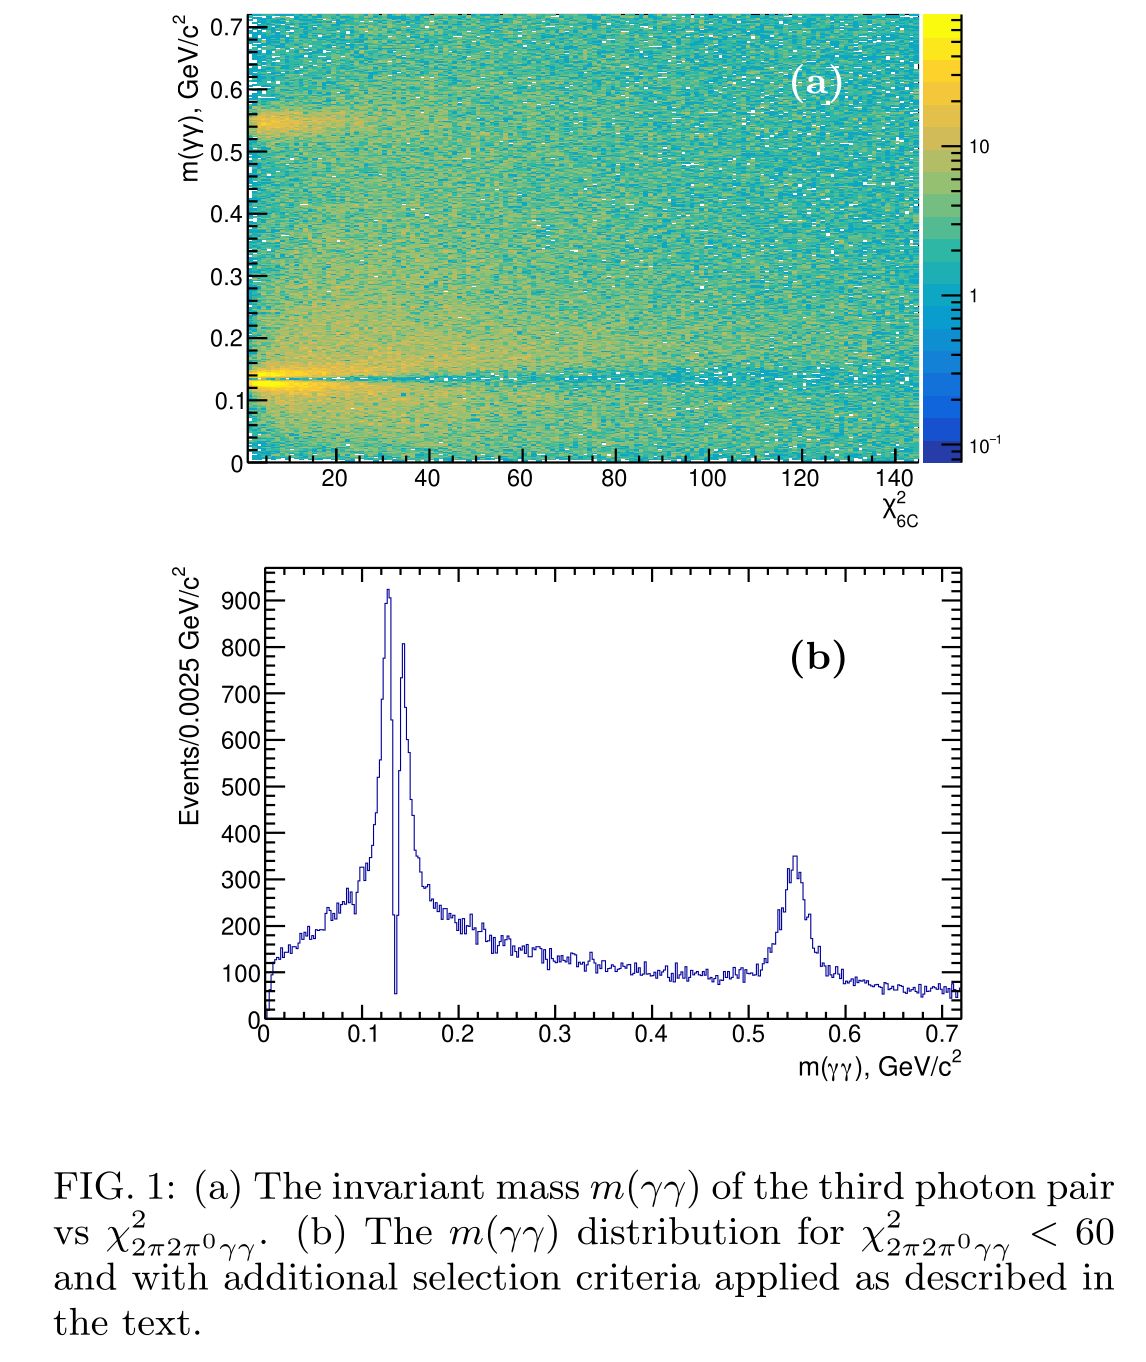
\includegraphics[height=.8\textheight]{figures/003/fig001}
  \hspace{5ex}
  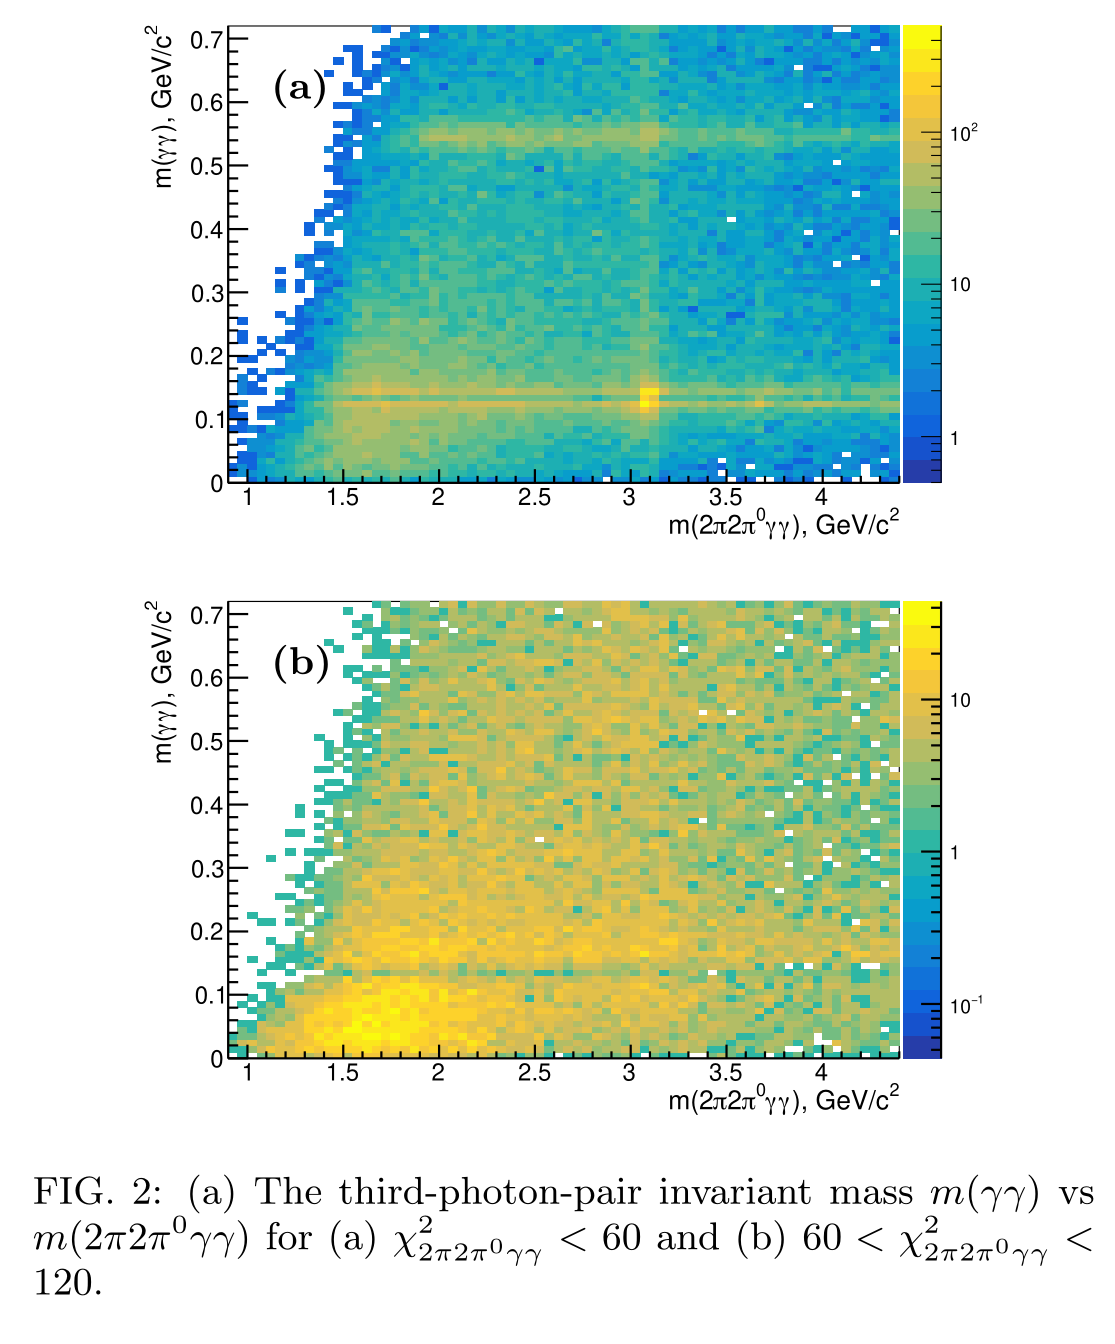
\includegraphics[height=.8\textheight]{figures/003/fig002}
\end{frame}%}}}

\begin{frame}[label=3pi-simulation]%{{{
  \frametitle{$\pip\pim3\piz$: simulation}
  \centering

  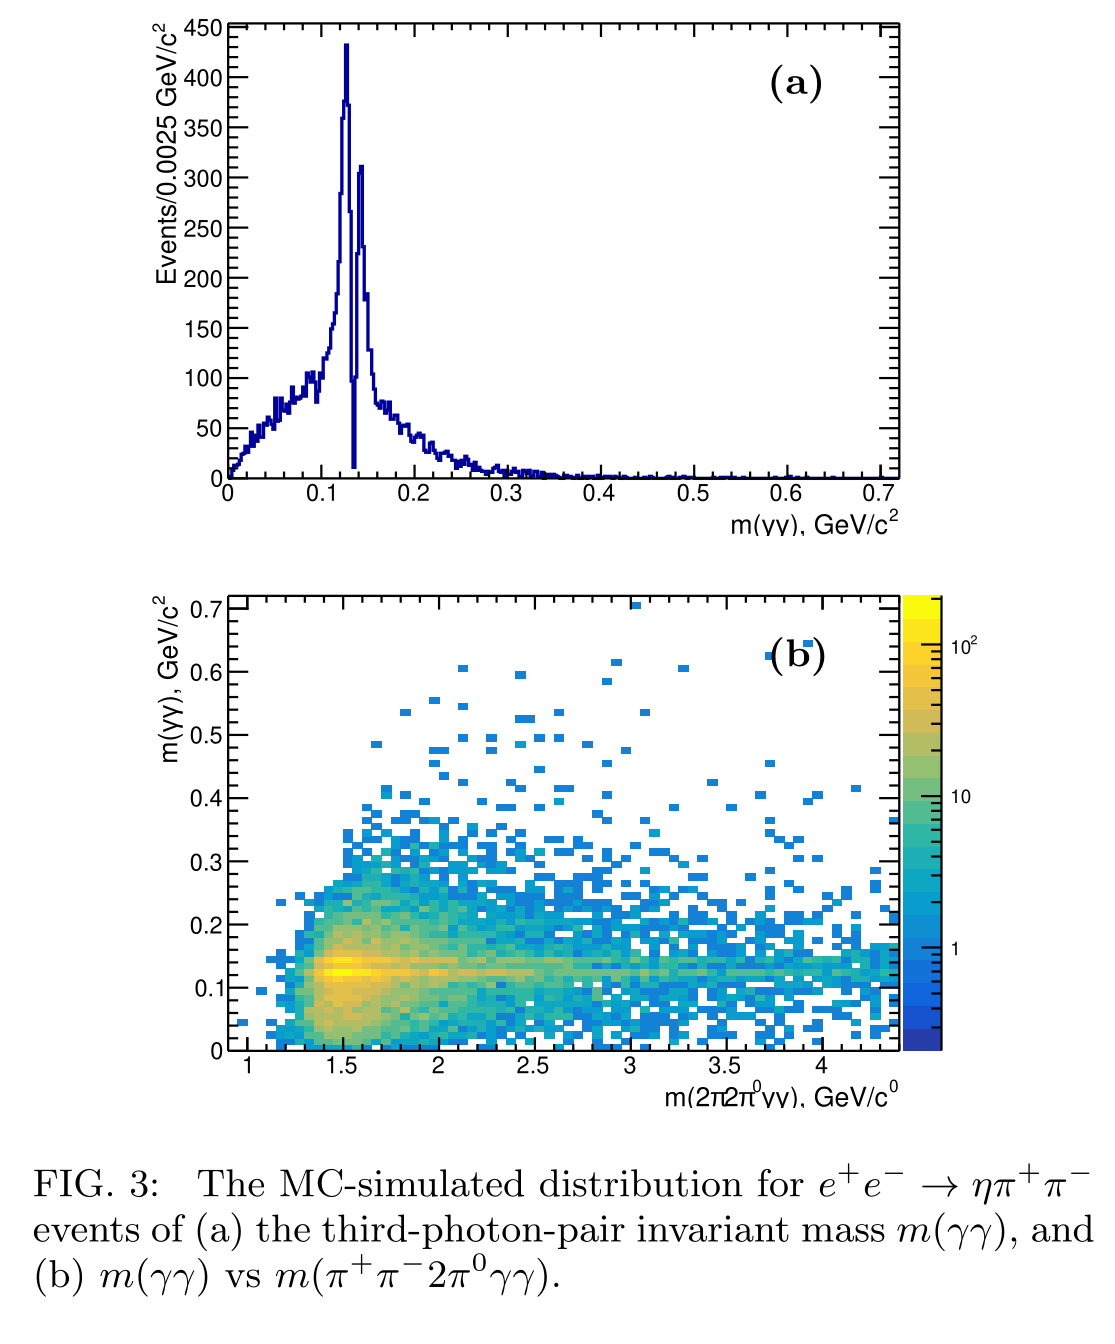
\includegraphics[height=.8\textheight]{figures/003/fig003}
  \hspace{5ex}
  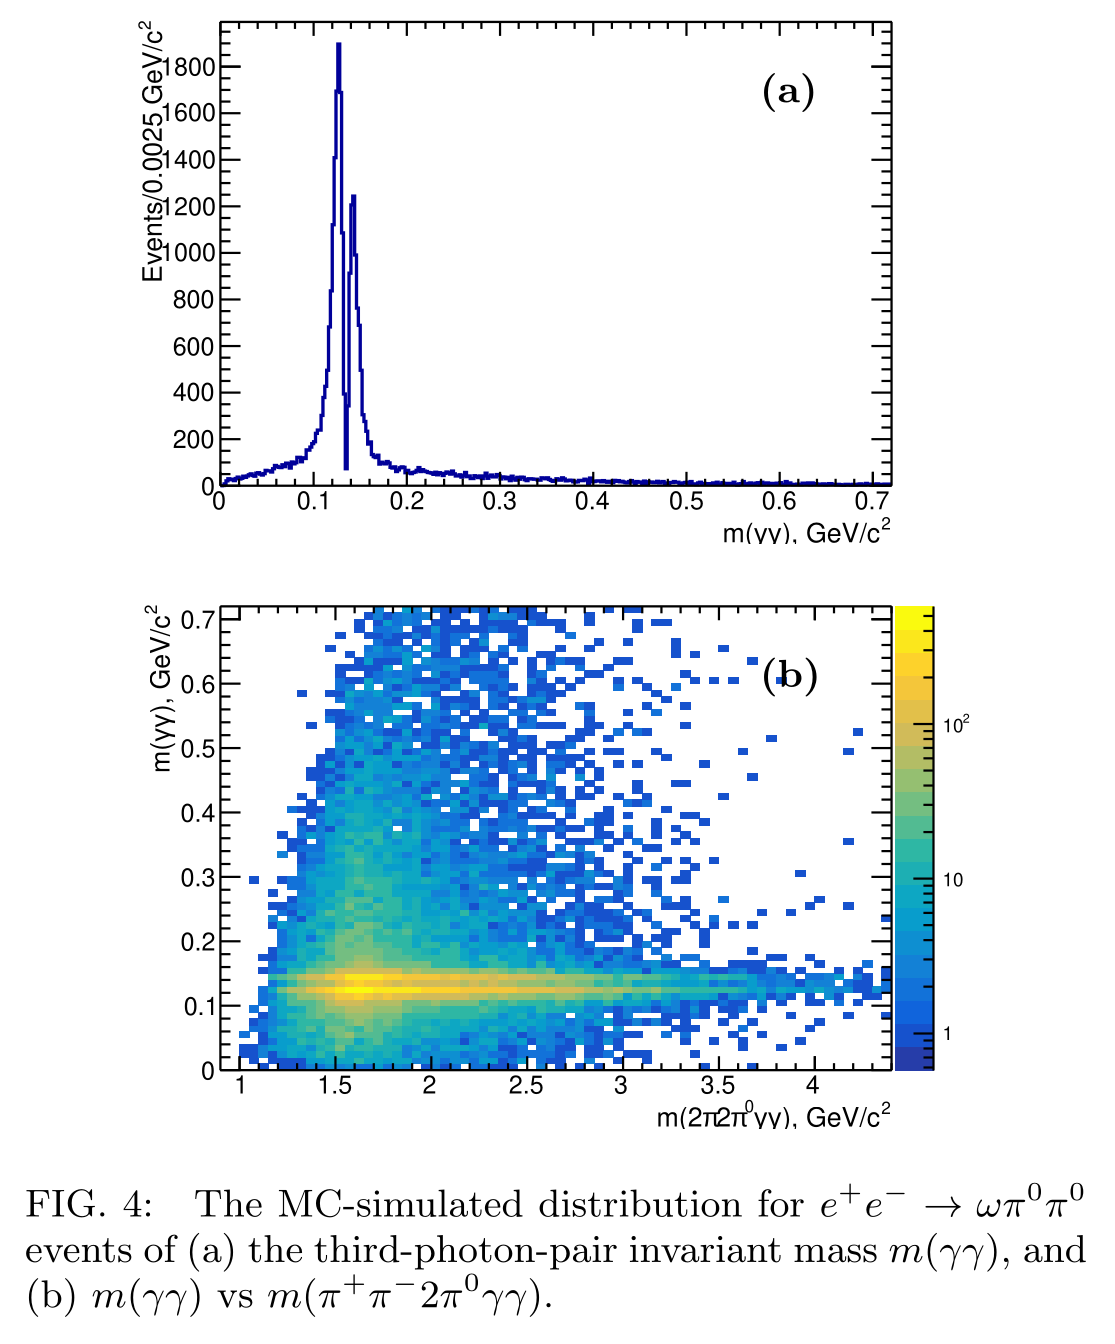
\includegraphics[height=.8\textheight]{figures/003/fig004}
\end{frame}%}}}

\begin{frame}[label=3pi-eff]%{{{
  \frametitle{$\pip\pim3\piz$: mass-dependent efficiency}
  \centering

  For bins in $m(2\pi2\piz\gamma\gamma)$ \\[1ex]

  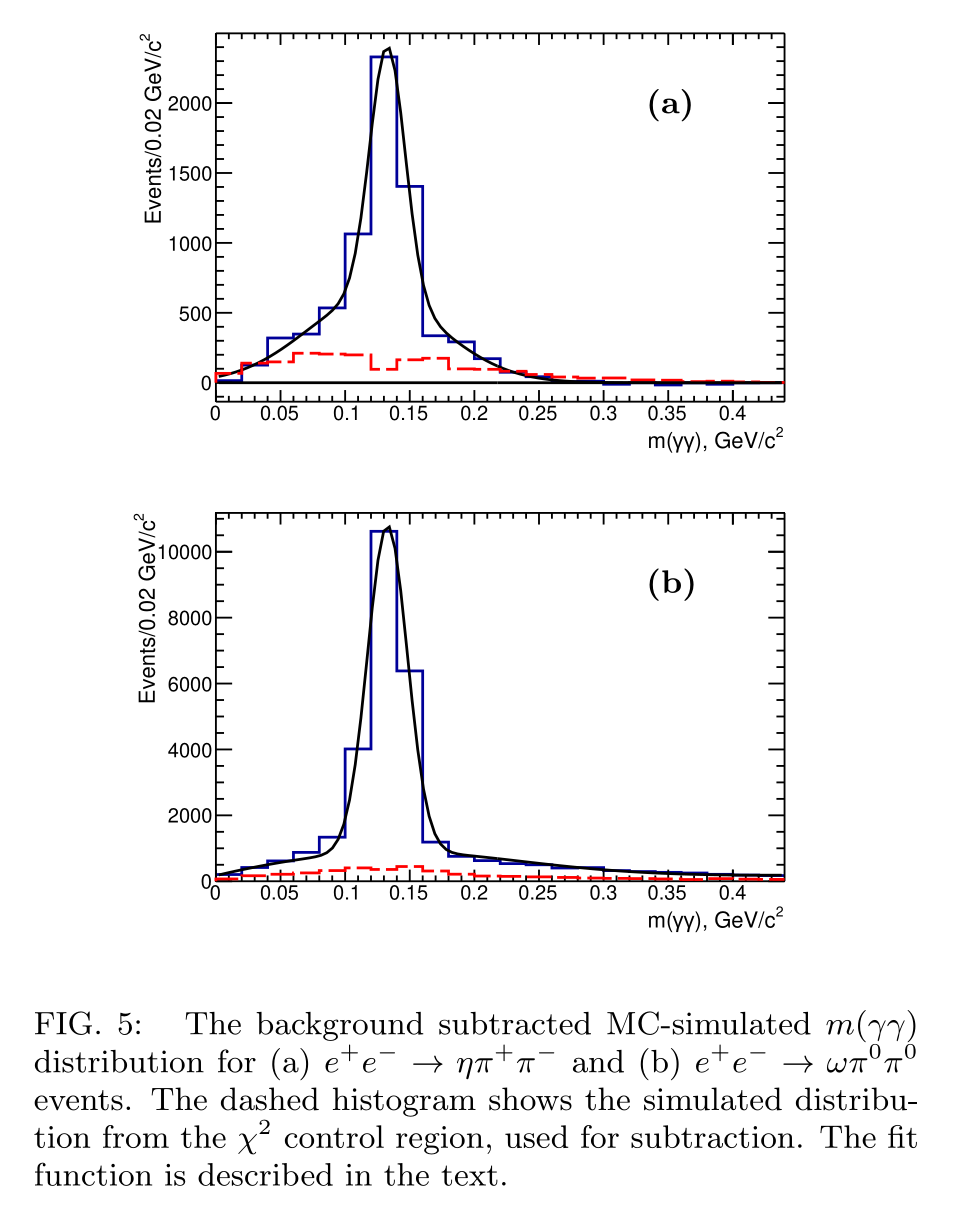
\includegraphics[width=.32\textwidth]{figures/003/fig005}
  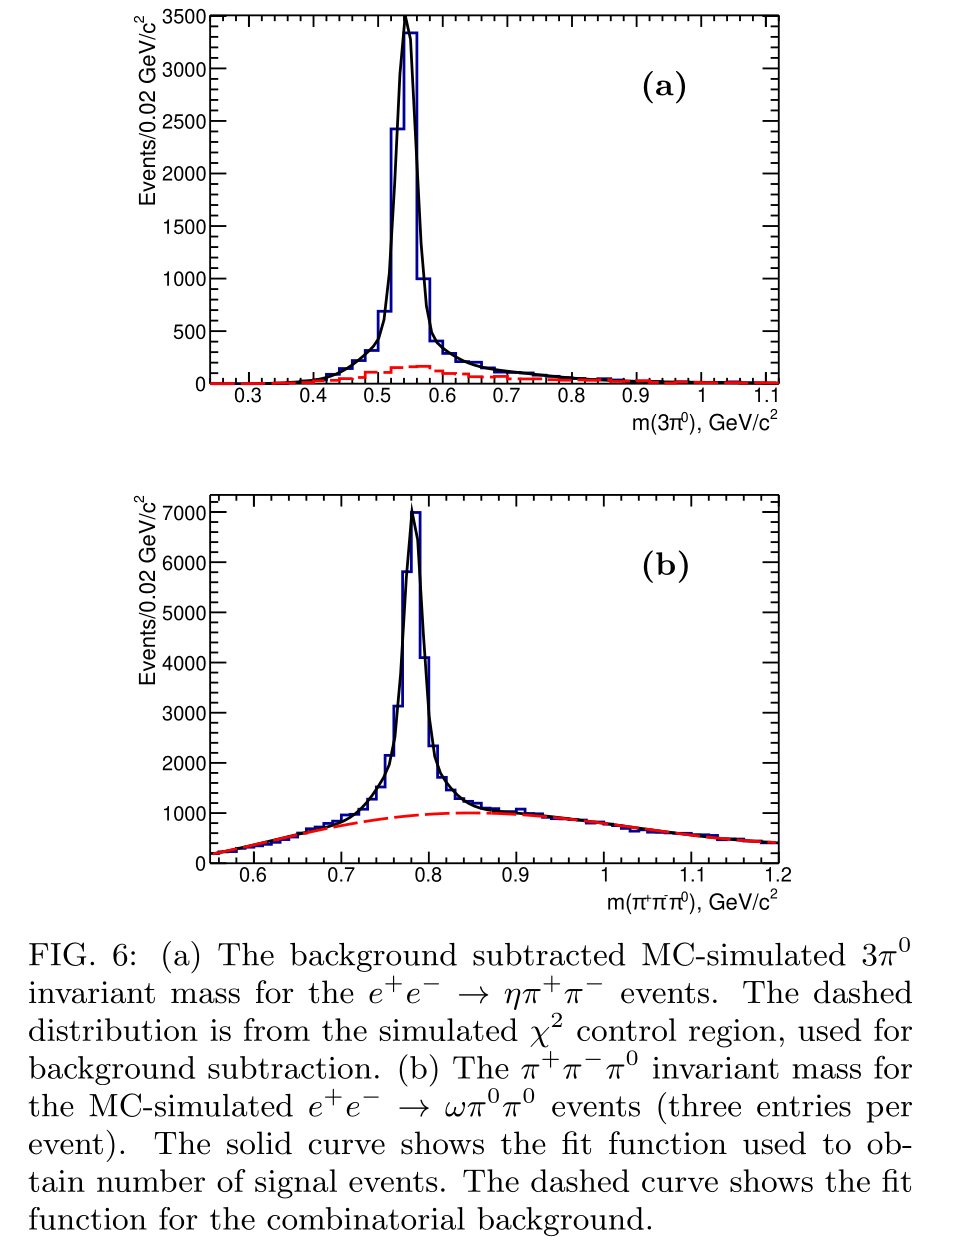
\includegraphics[width=.32\textwidth]{figures/003/fig006}
  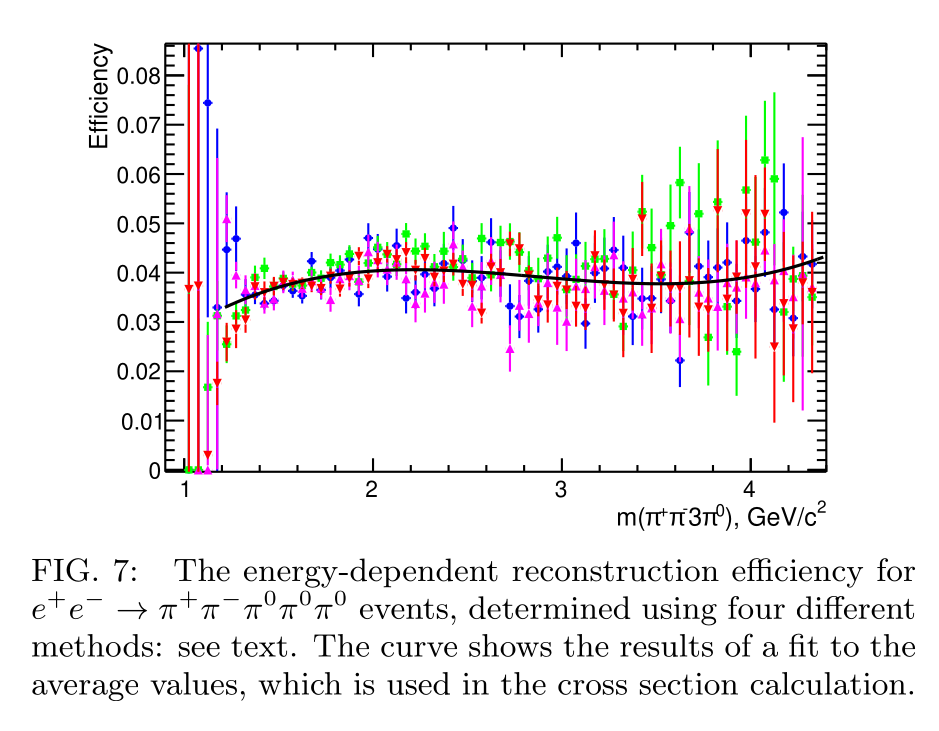
\includegraphics[width=.32\textwidth]{figures/003/fig007}
\end{frame}%}}}

\begin{frame}[label=3pi-signal]%{{{
  \frametitle{$\pip\pim3\piz$: signal yields per 
  $m(2\pi2\piz\gamma\gamma)$ bins}
  \centering

  $14\,390 \pm 182$ in total \\[1ex]

  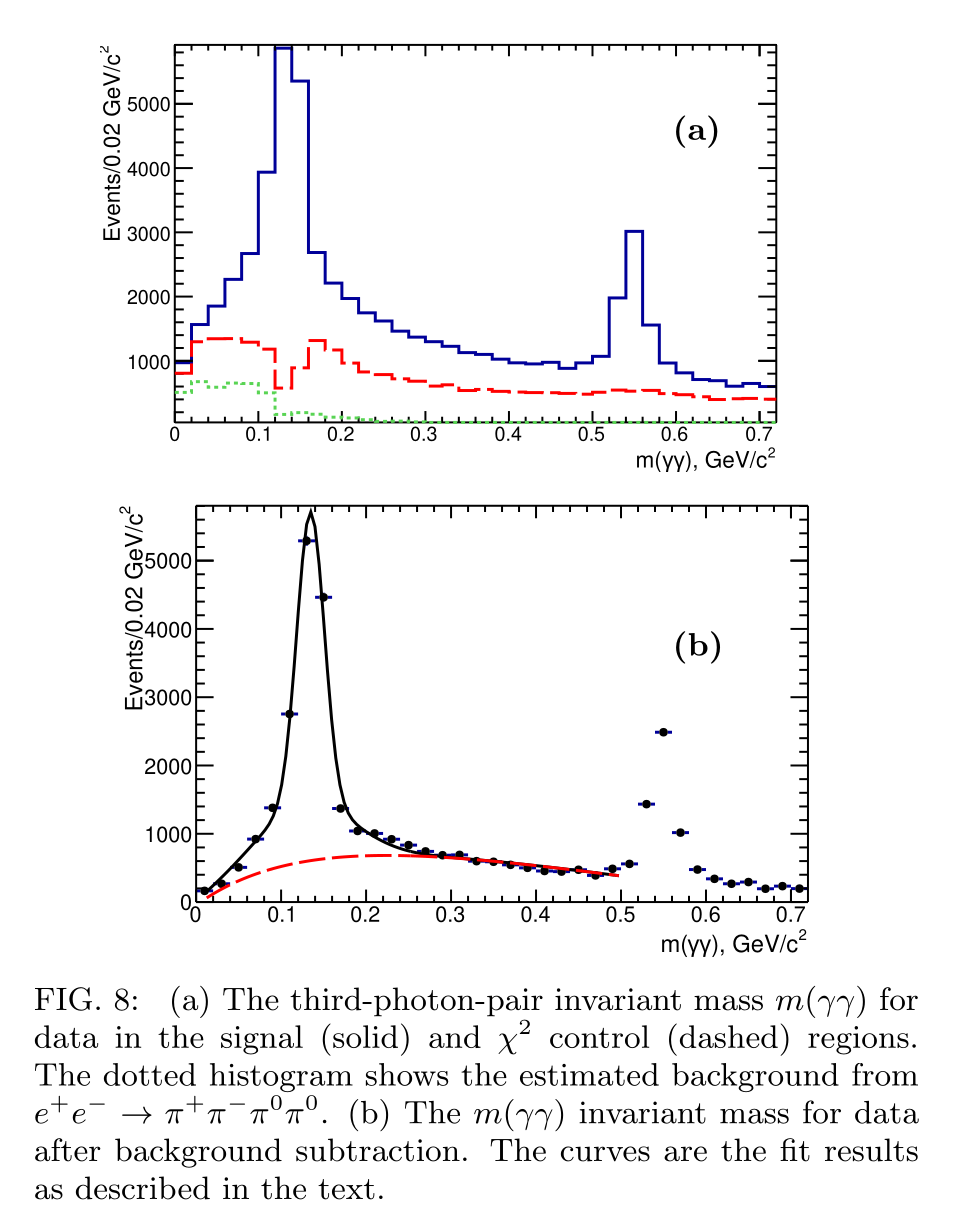
\includegraphics[width=.35\linewidth]{figures/003/fig008}
  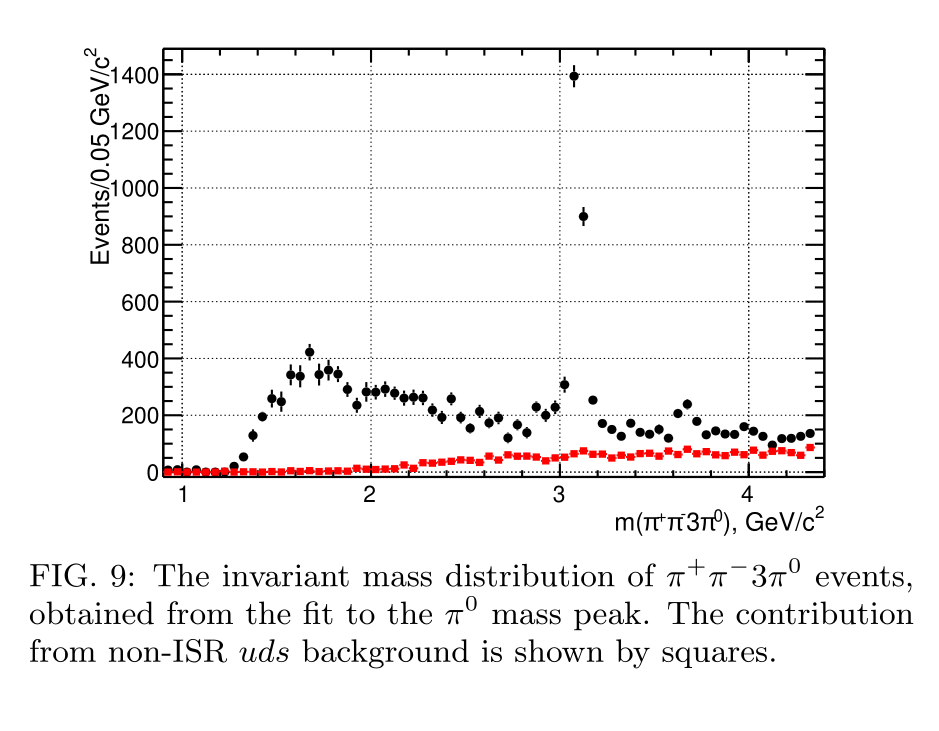
\includegraphics[width=.5\linewidth]{figures/003/fig009}
\end{frame}%}}}

\begin{frame}[label=3pi-bkg]%{{{
  \frametitle{$\pip\pim3\piz$: peaking background from non-ISR events}
  \centering

  $ee\to\pip\pim3\piz\piz$ with $\piz\to2\gamma$, one $\gamma$ very hard
  \\[1ex]

  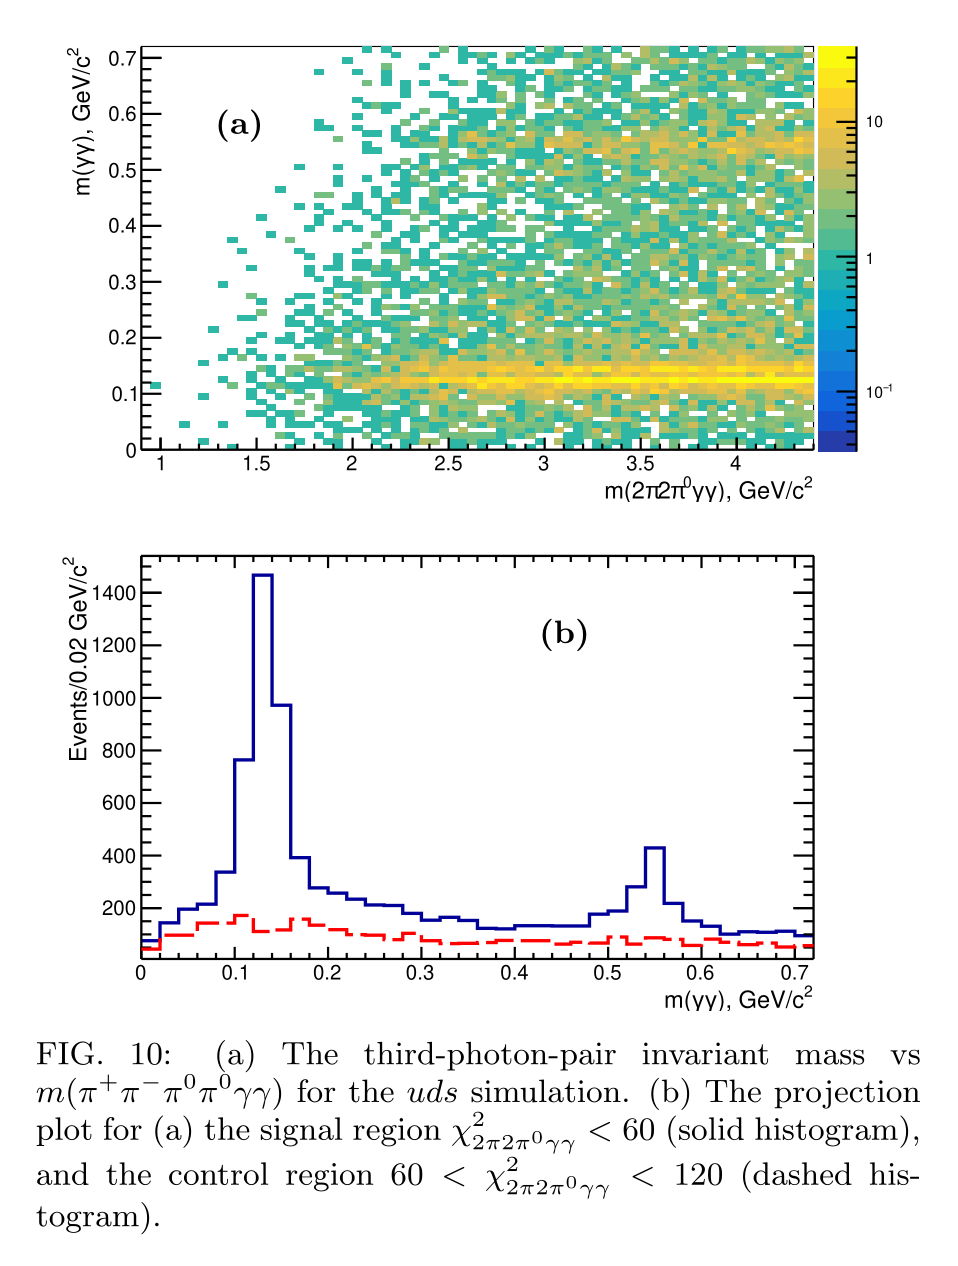
\includegraphics[width=.33\linewidth]{figures/003/fig010}
  \parbox[b]{.6\textwidth}{
    $ \sigma(2\pi3\piz)(E_\text{c.m.}) = \dfrac{\mathrm{d}
    N_{5\pi\gamma}(E_\text{c.m.})}
    {\mathrm{d}\mathcal{L}(E_\text{c.m.})
    \varepsilon^\text{corr}_{5\pi}
    \varepsilon^\text{MC}_{5\pi}(E_\text{c.m.})
    (1 + \delta_R)}$ \\
    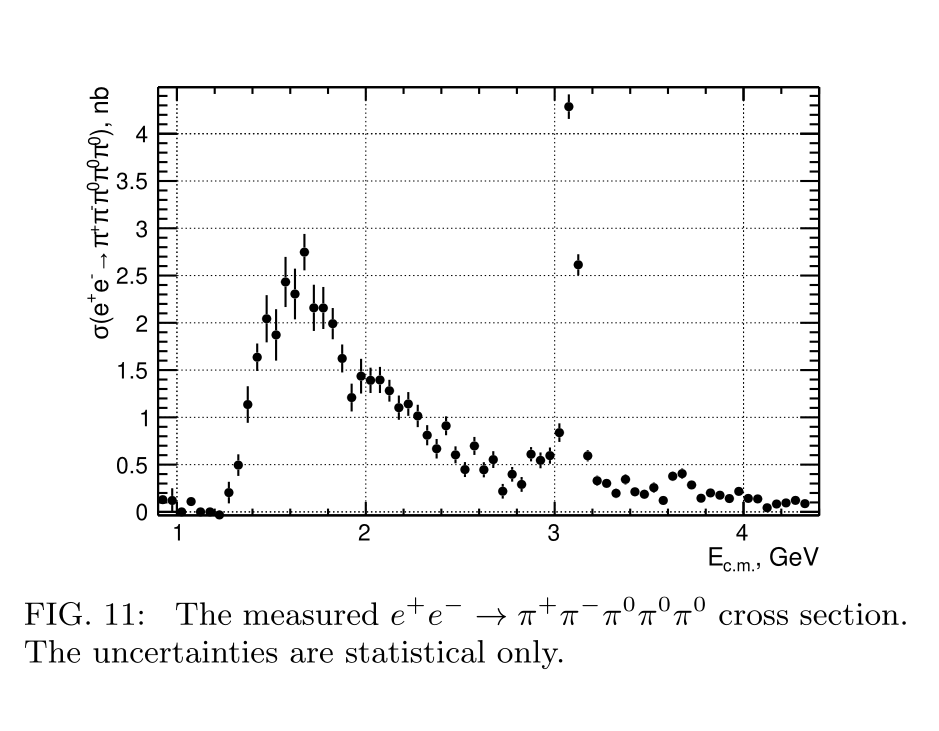
\includegraphics[width=.5\textwidth]{figures/003/fig011}
  }
\end{frame}%}}}

\begin{frame}[label=3pi-res-eta]%{{{
  \frametitle{$\pip\pim3\piz$: resonant structure: $\eta\to3\piz$}
  \centering

  $\eta\to3\piz$ peak, $\pip\pim$ coming from $\rho(770)$ \\[1ex]

  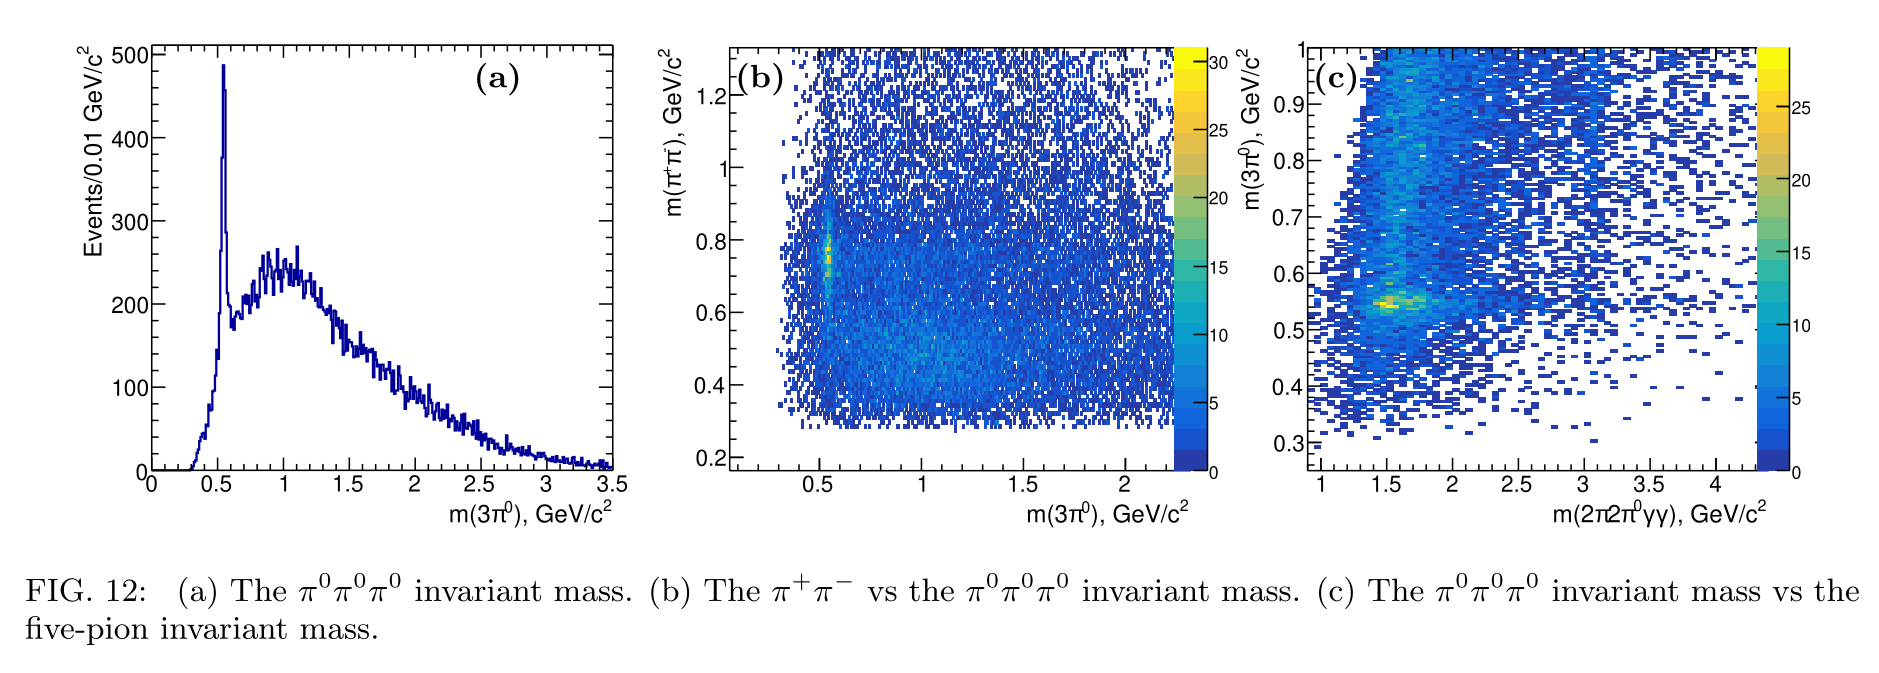
\includegraphics[width=\linewidth]{figures/003/fig012}
\end{frame}%}}}

\begin{frame}[label=3pi-res-eta]%{{{
  \frametitle{$\pip\pim3\piz$: resonant structure: $\eta\to3\piz$}
  \centering

  $2102 \pm 112$ in total \\
  $\rho$ visible in $\eta$ range, much less in sidebands \\[1ex]

  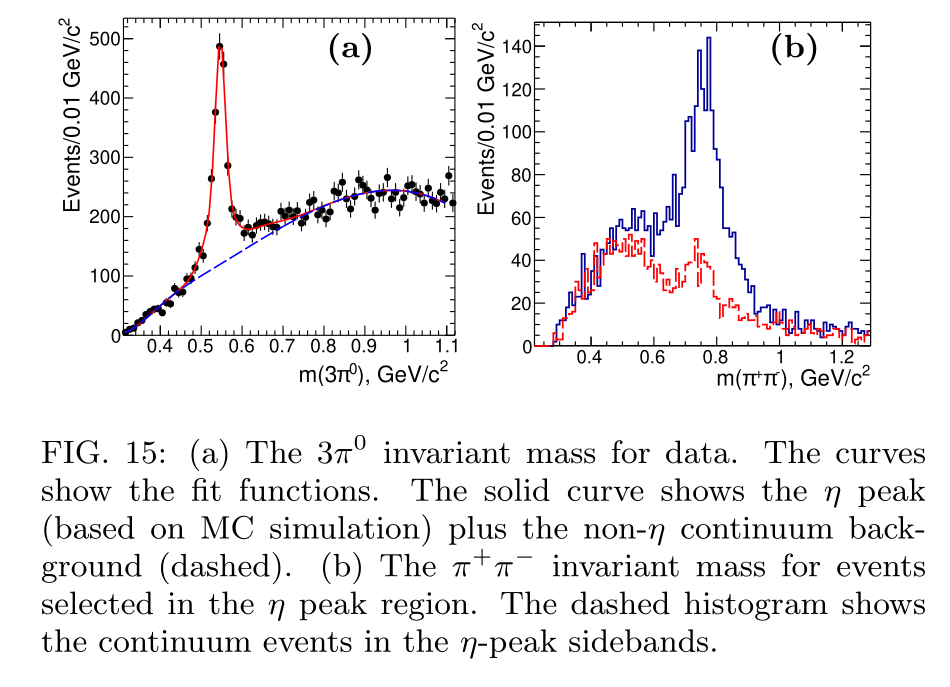
\includegraphics[width=.42\linewidth]{figures/003/fig015}
  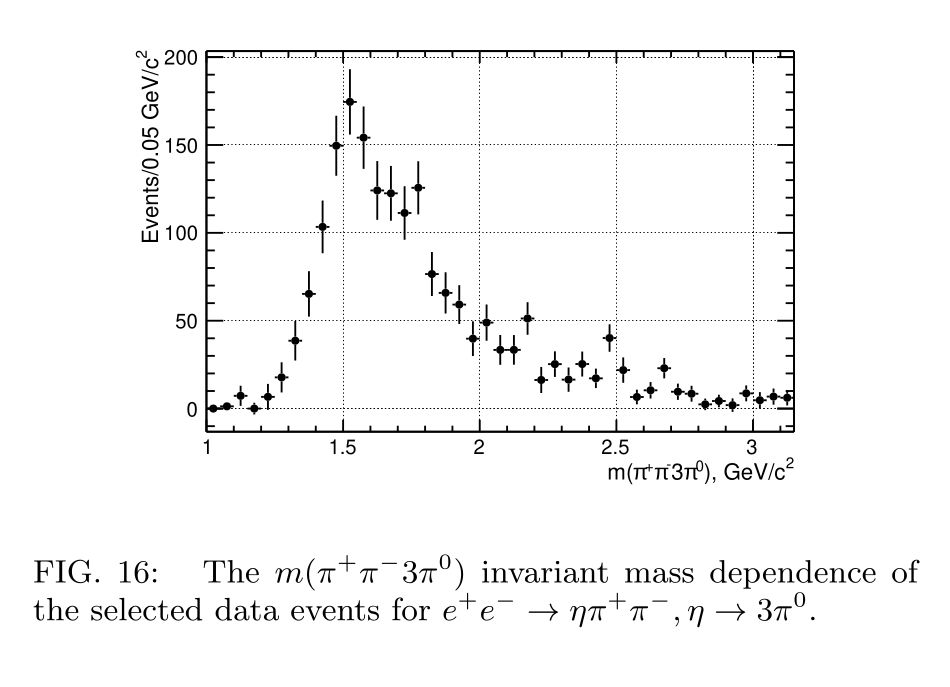
\includegraphics[width=.34\linewidth]{figures/003/fig016}
  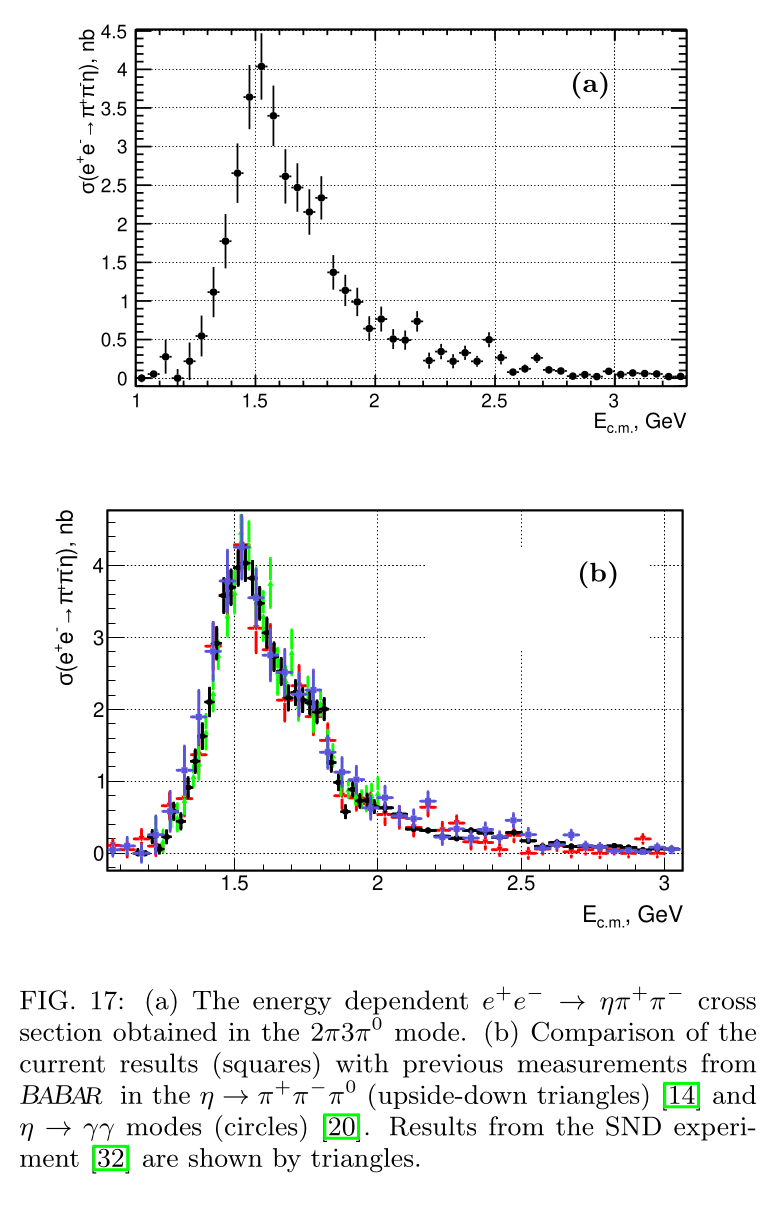
\includegraphics[width=.22\linewidth]{figures/003/fig017}
\end{frame}%}}}

\begin{frame}[label=3pi-res-omega]%{{{
  \frametitle{$\pip\pim3\piz$: resonant structure: $\omega\to\pip\pim\piz$}
  \centering

  $\omega\to\pip\pim\piz$ peak, indications of $\phi$, $J/\psi$ \\[1ex]

  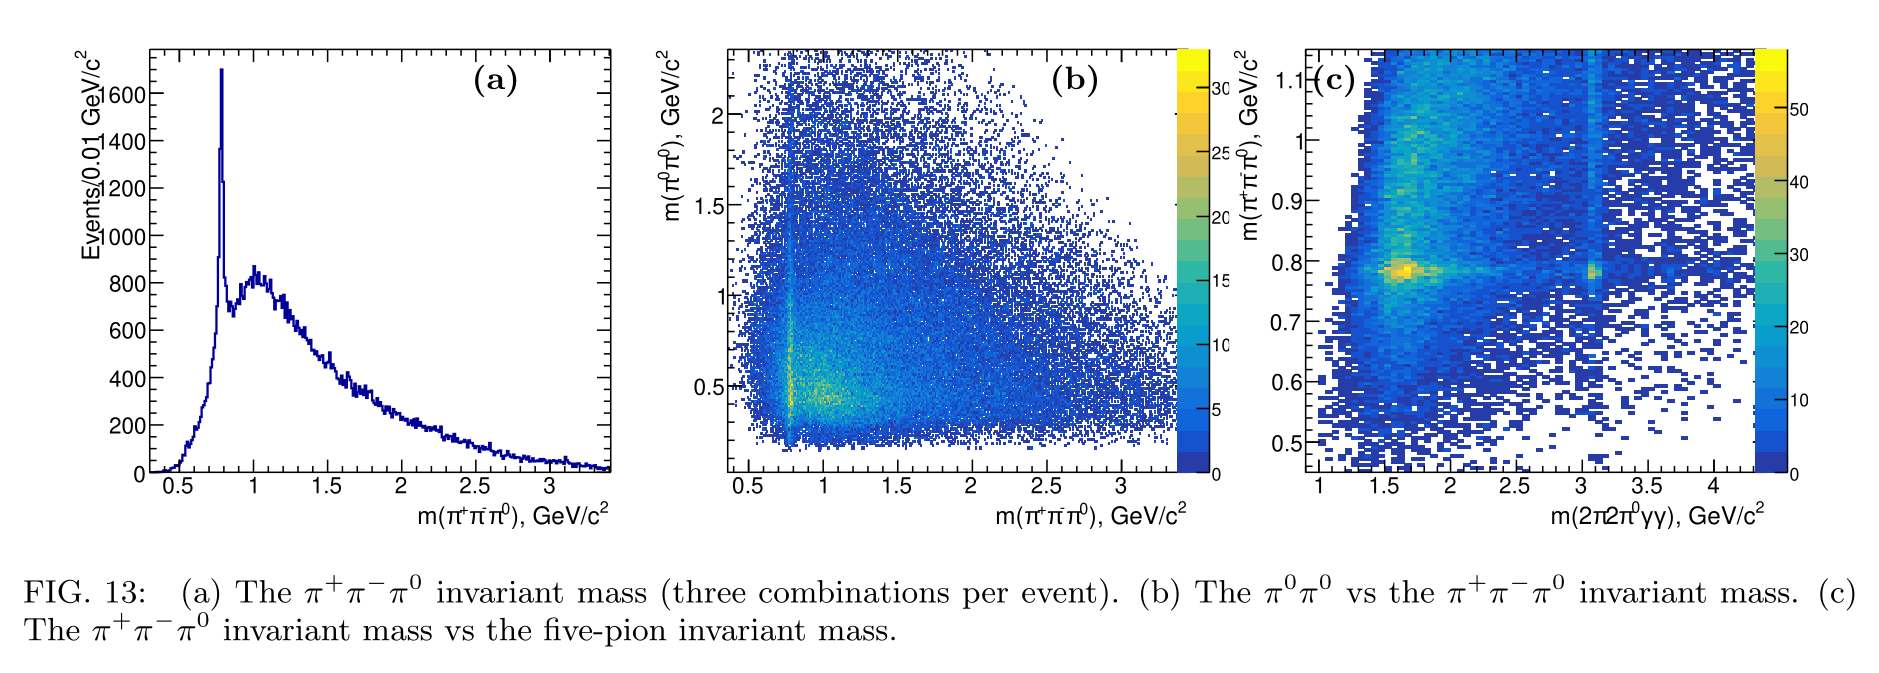
\includegraphics[width=\linewidth]{figures/003/fig013}
\end{frame}%}}}

\begin{frame}[label=3pi-res-omega]%{{{
  \frametitle{$\pip\pim3\piz$: resonant structure: $\omega\to\pip\pim\piz$}
  \centering

  $3960 \pm 146$ events in total,
  $f_0(980)$ not clearly visible in $m(\piz\piz)$,
  $\omega(1650)$ contribution \\
  Cross-section 2 times smaller than $ee\to\omega\pip\pim$, as expected 
  from isospin symmetry \\[1ex]

  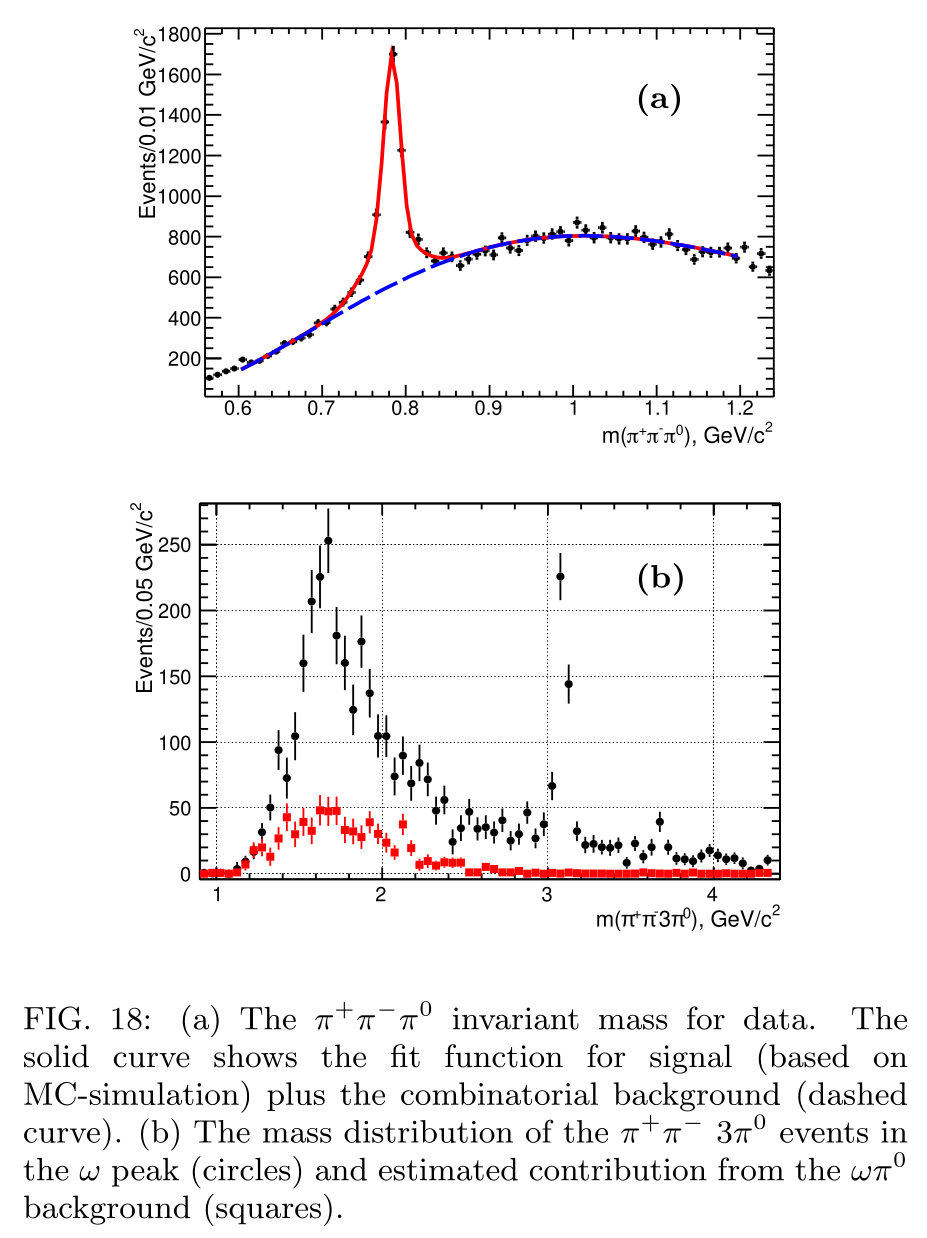
\includegraphics[width=.3\linewidth]{figures/003/fig018}
  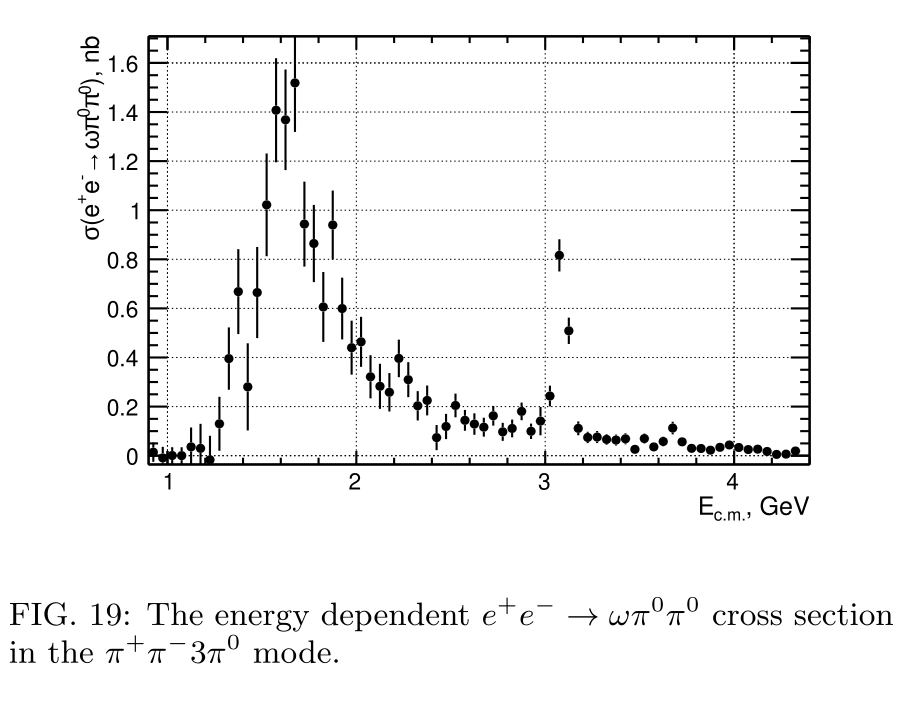
\includegraphics[width=.5\linewidth]{figures/003/fig019}
\end{frame}%}}}

\begin{frame}[label=3pi-res-rho]%{{{
  \frametitle{$\pip\pim3\piz$: resonant structure: $\rho^\pm\to\pi^\pm\piz$}
  \centering

  $\rho\to\pi\piz$ peak, intermediate $\rhop\rhom\piz$ \\
  Clear $J/\psi$ and indication of $\psi(2S)$ \\[1ex]

  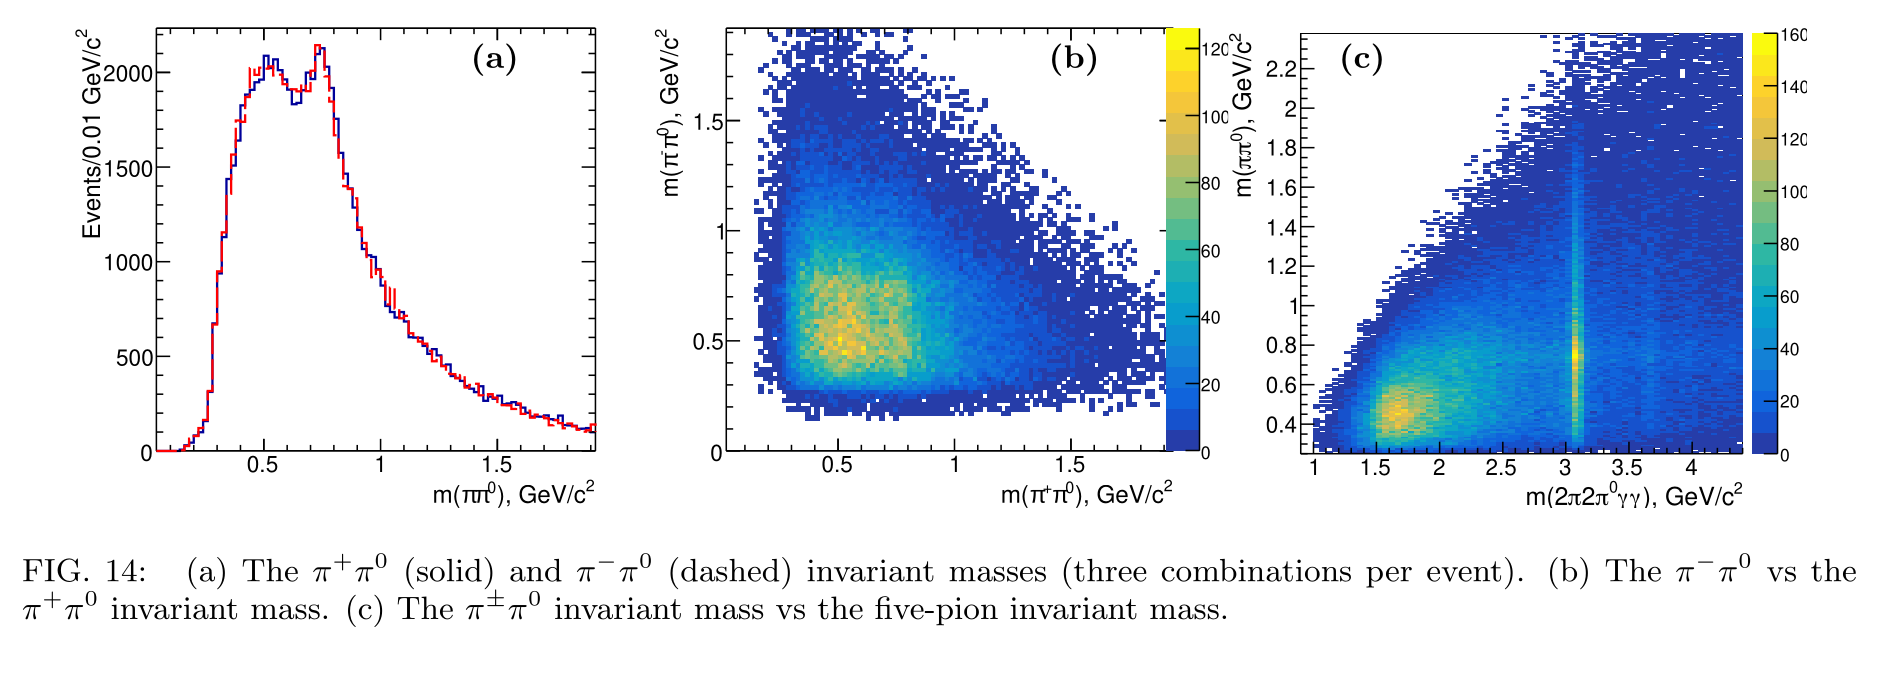
\includegraphics[width=\linewidth]{figures/003/fig014}
\end{frame}%}}}

\begin{frame}[label=3pi-res-rho]%{{{
  \frametitle{$\pip\pim3\piz$: resonant structure: $\rho^\pm\to\pi^\pm\piz$}
  \centering

  \parbox[b]{.68\textwidth}{
  $14\,894 \pm 501$ events in total, \\ correlated $\rhop\rhom\piz$ 
  production decreases with $m(5\pi)$ \\
  Statistics not significant for $\rho$ decays resonant 
  sub-sub-structure \\[1ex]
  Sum of intermediate states does give the full cross-section \\[1ex]
    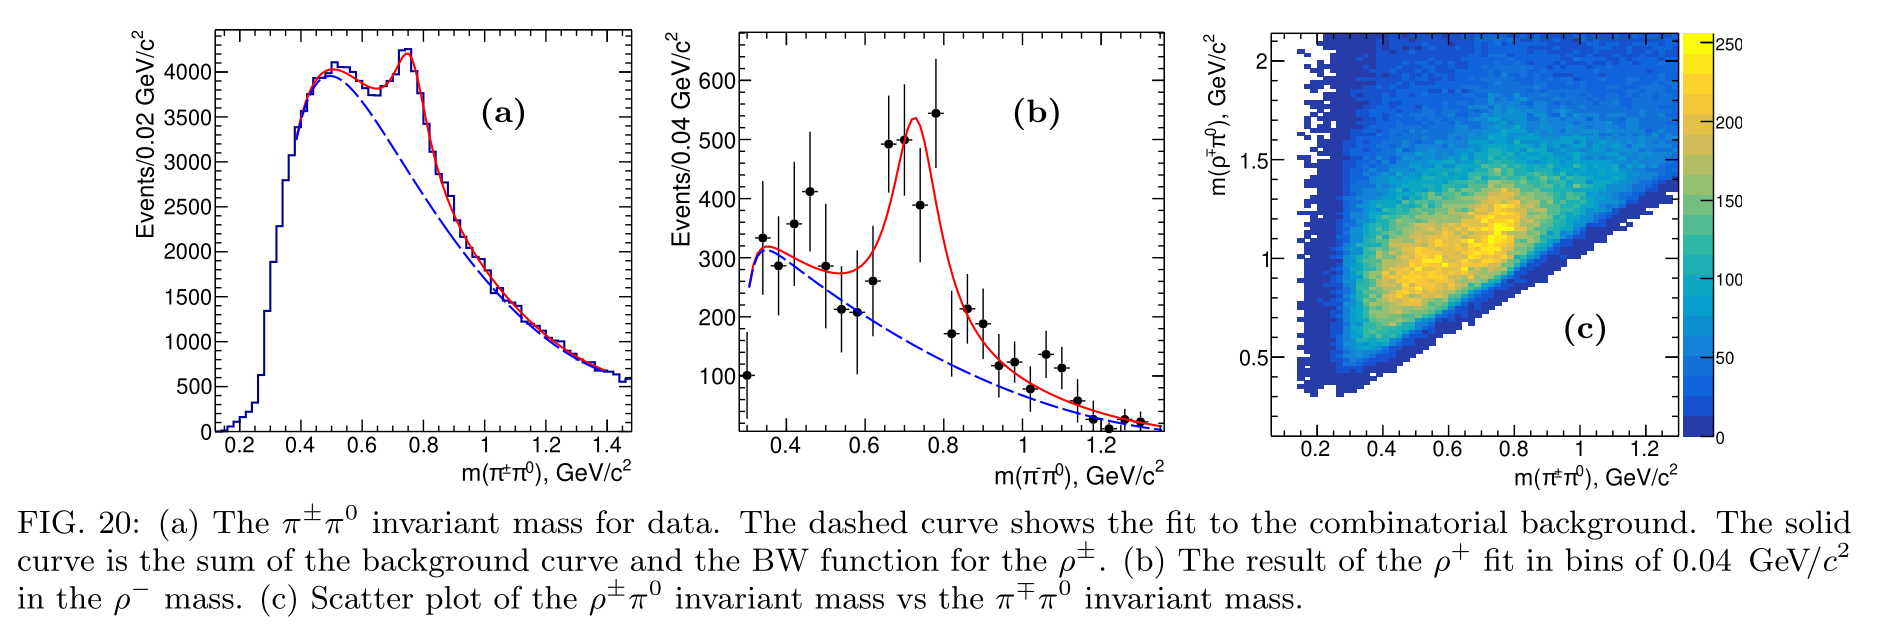
\includegraphics[width=.68\textwidth]{figures/003/fig020}
  }
  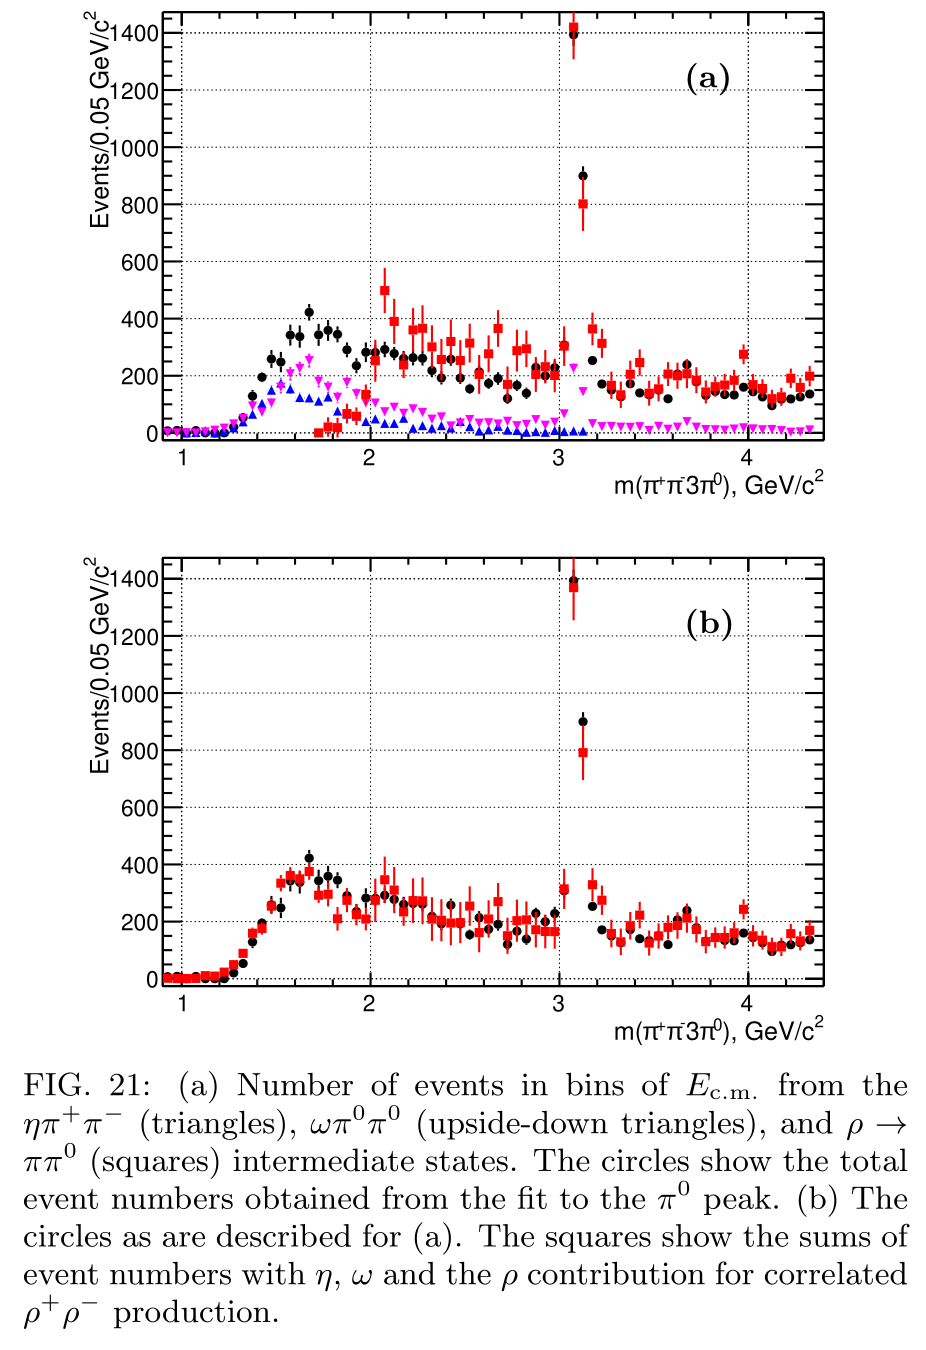
\includegraphics[width=.3\linewidth]{figures/003/fig021}
\end{frame}%}}}

\begin{frame}[label=2pieta-signal]%{{{
  \frametitle{$\pip\pim2\piz\eta$: signal yields per 
  $m(2\pi2\piz\gamma\gamma)$ bins}
  \centering

  $4700 \pm 84$ events in total \\[1ex]

  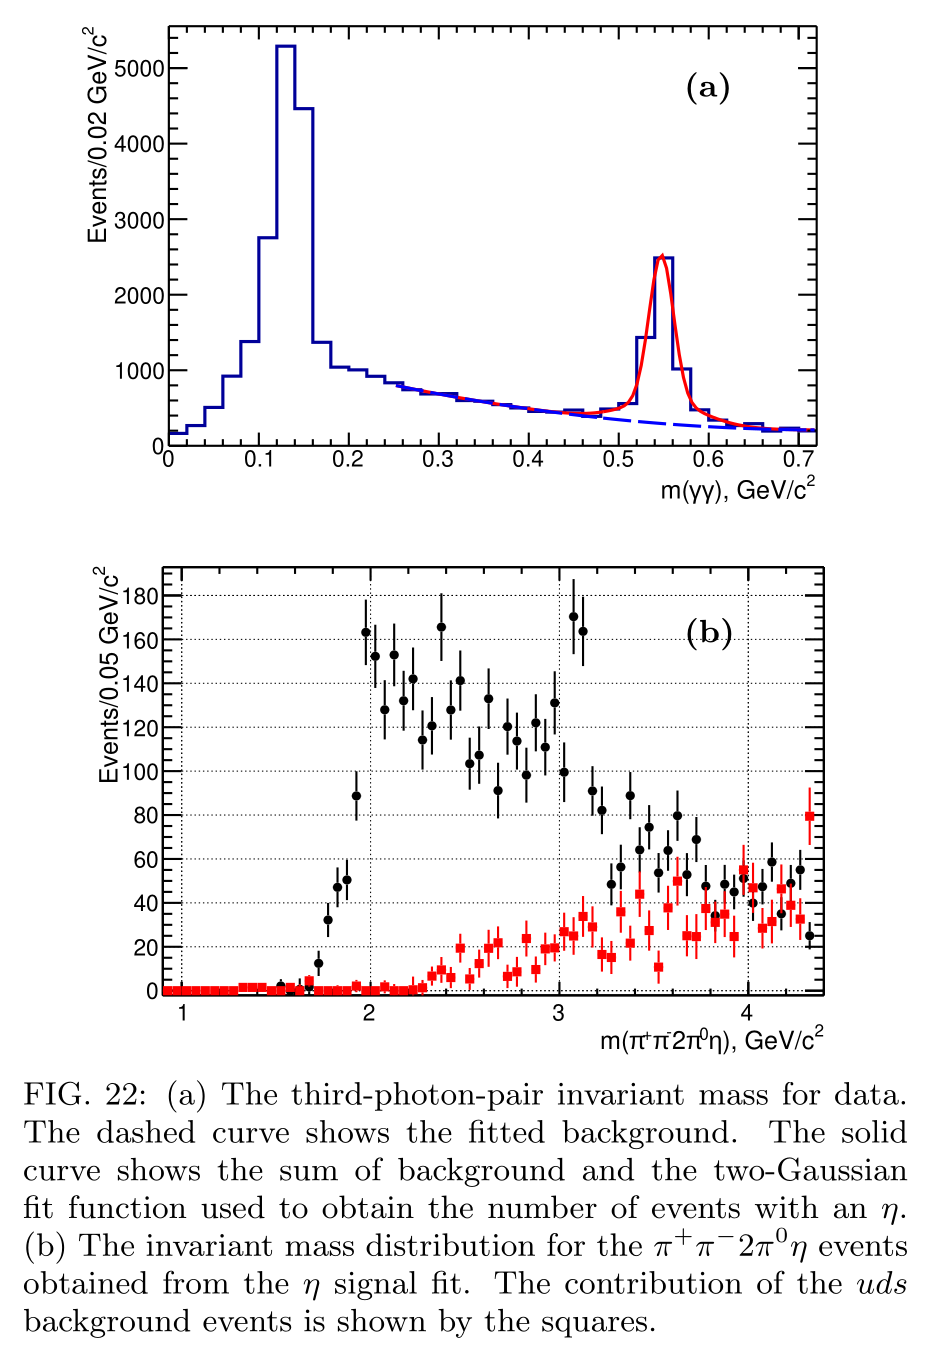
\includegraphics[width=.3\textwidth]{figures/003/fig022}
\end{frame}%}}}

\begin{frame}[label=2pieta-eff]%{{{
  \frametitle{$\pip\pim2\piz\eta$: mass-dependent efficiency}
  \centering

  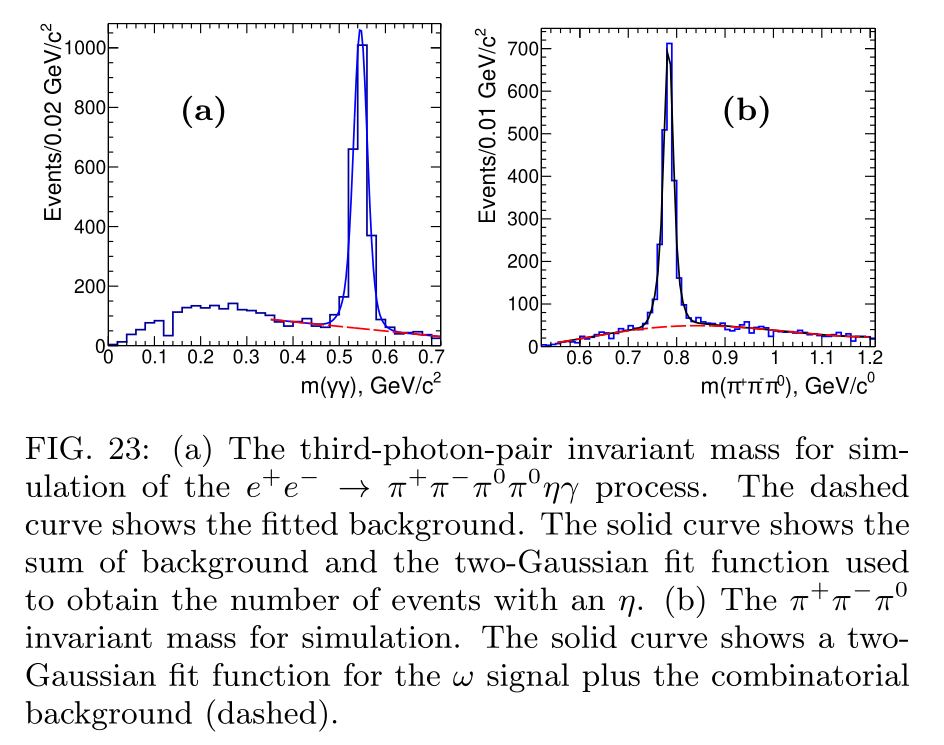
\includegraphics[width=.48\textwidth]{figures/003/fig023}
  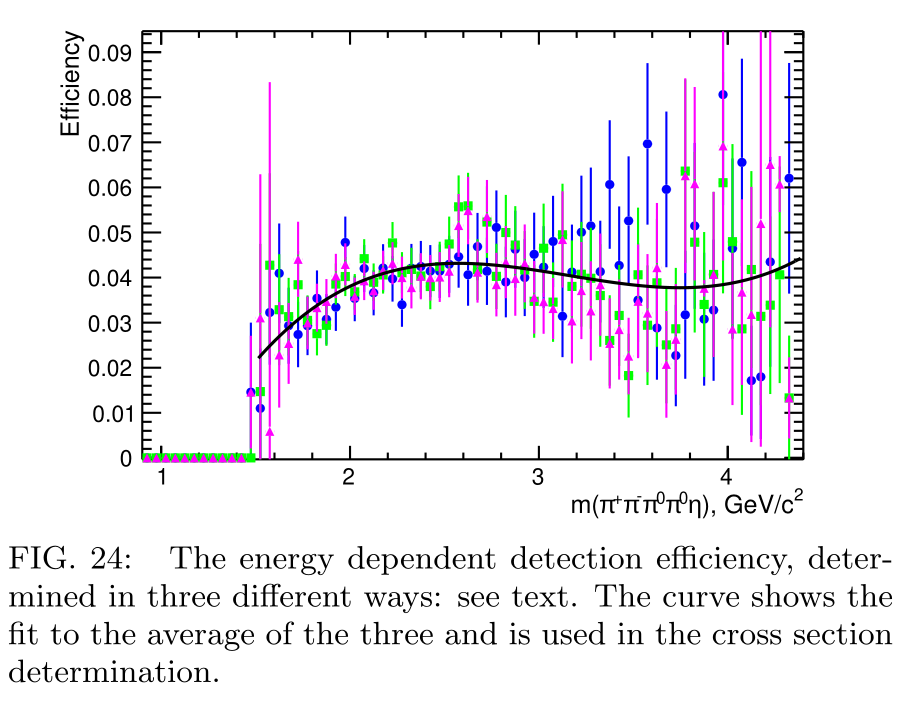
\includegraphics[width=.48\textwidth]{figures/003/fig024}
\end{frame}%}}}

\begin{frame}[label=2pieta-cross-section]%{{{
  \frametitle{$\pip\pim2\piz\eta$: cross-section}
  \centering

  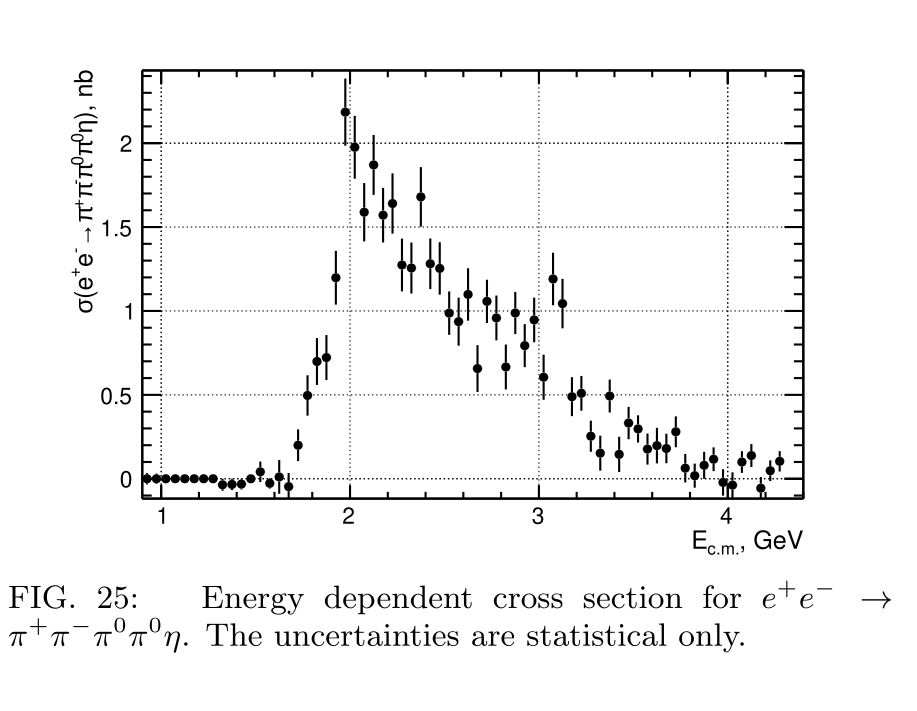
\includegraphics[width=.48\textwidth]{figures/003/fig025}
\end{frame}%}}}

\begin{frame}[label=2pieta-res-eta1285]%{{{
  \frametitle{$\pip\pim2\piz\eta$: resonant structure: tiny 
  $\eta(1285)\to\piz\piz\eta$}
  \centering

  $\eta(1285)$ small but clear compared to sideband (red). No major 
  structures \\[1ex]

  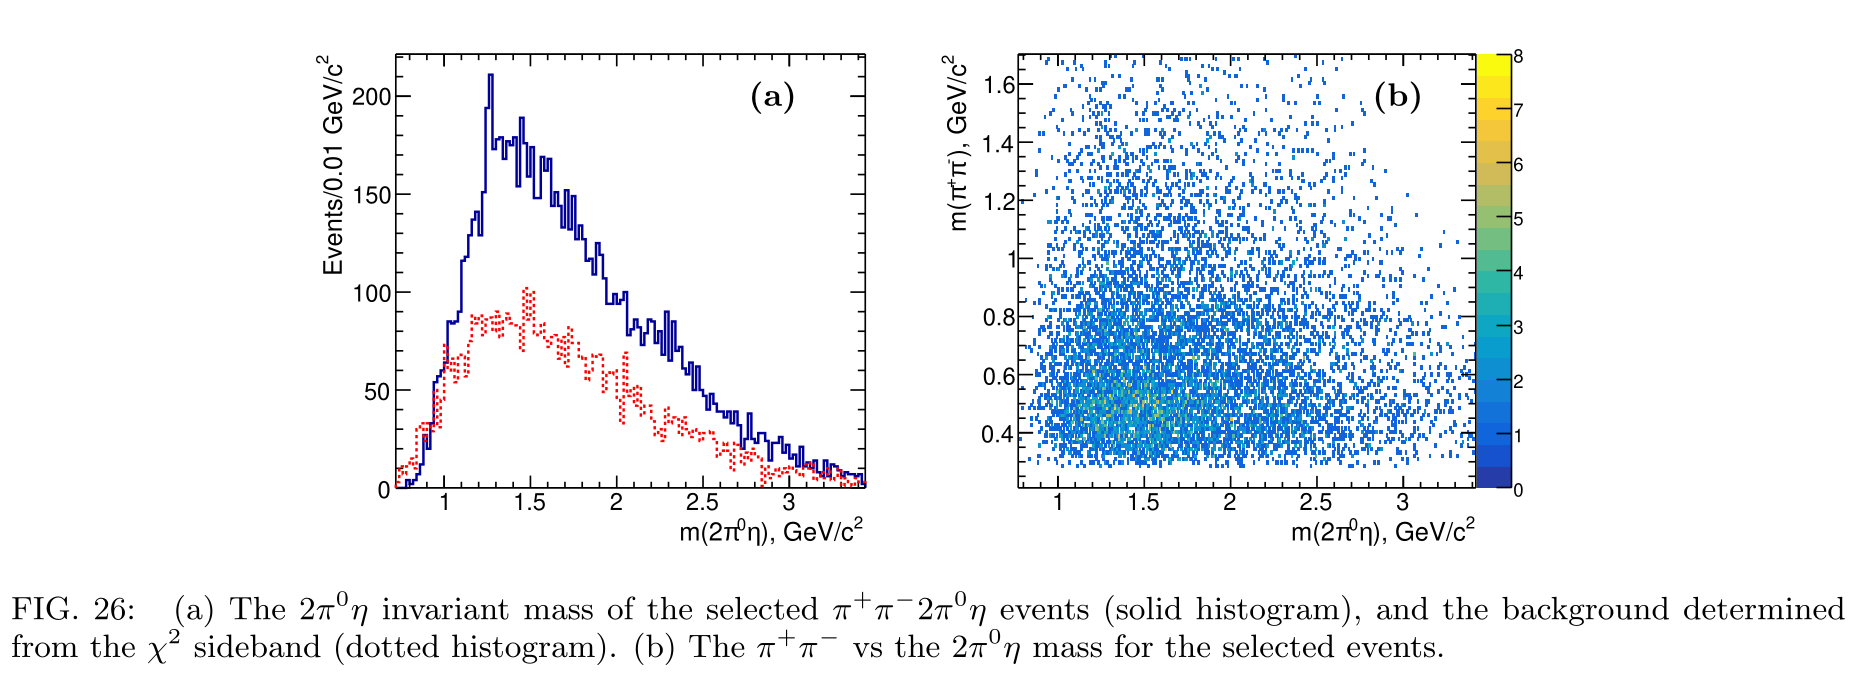
\includegraphics[width=\textwidth]{figures/003/fig026}
\end{frame}%}}}

\begin{frame}[label=2pieta-res-omega]%{{{
  \frametitle{$\pip\pim2\piz\eta$: resonant structure: 
  $\omega\to\pip\pim\piz$}
  \centering

  $\omega\to\pip\pim\piz$ huge peak, $\phi$ at 1 GeV \\
  $a_0(980)\to\eta\piz$ correlation with $\omega$ \\[1ex]

  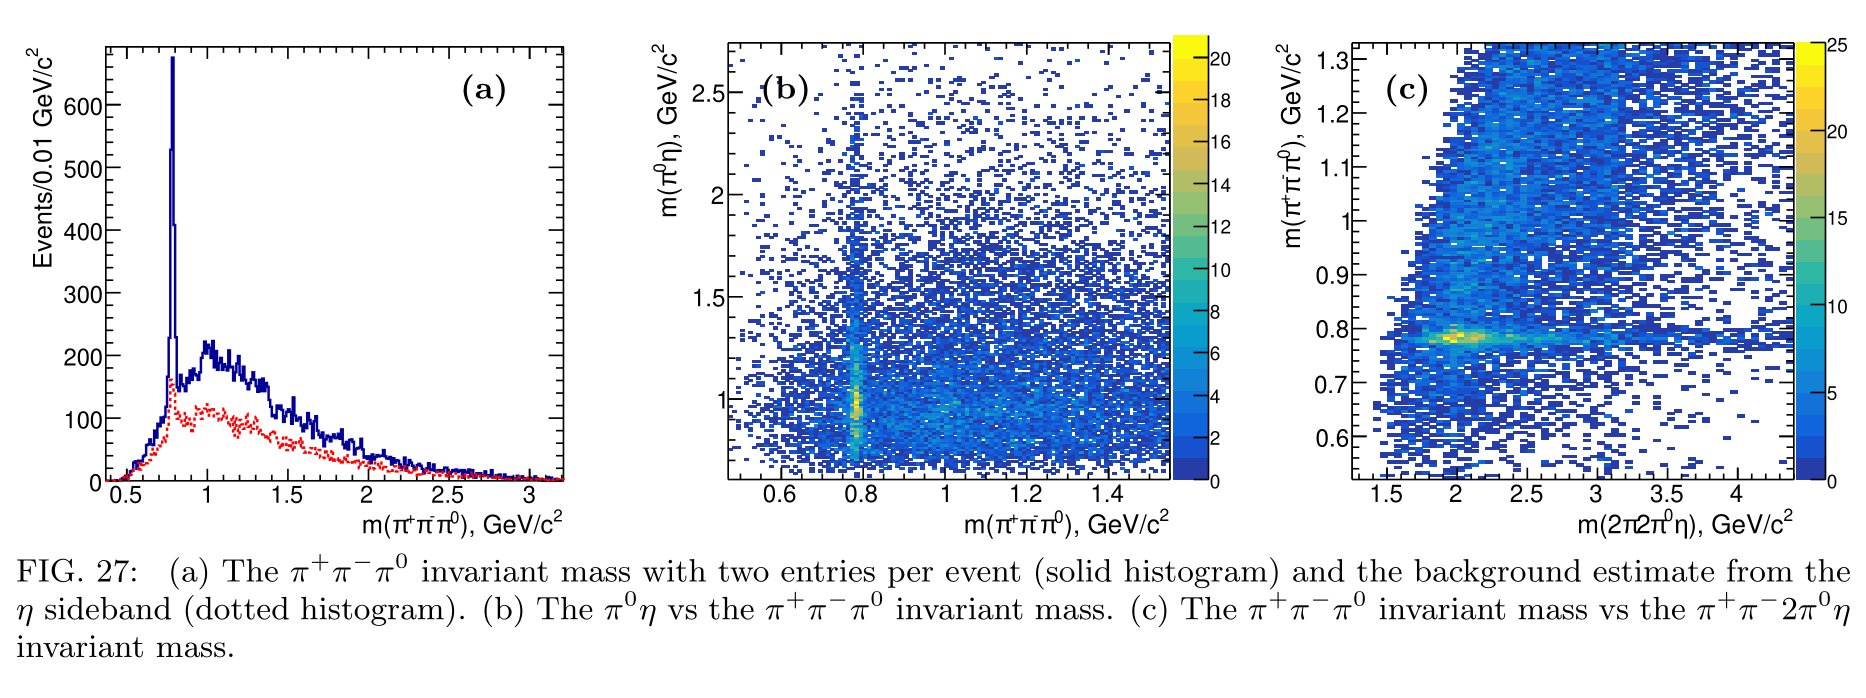
\includegraphics[width=\textwidth]{figures/003/fig027}
\end{frame}%}}}

\begin{frame}[label=2pieta-res-omega]%{{{
  \frametitle{$\pip\pim2\piz\eta$: resonant structure: 
  $\omega\to\pip\pim\piz$}
  \centering

  $1676 \pm 22$ events for $\omega$ and $269 \pm 68$ events for $\phi$ \\
  Clear $a_0(980)$ in $\omega$ peak but not its sidebands \\[1ex]

  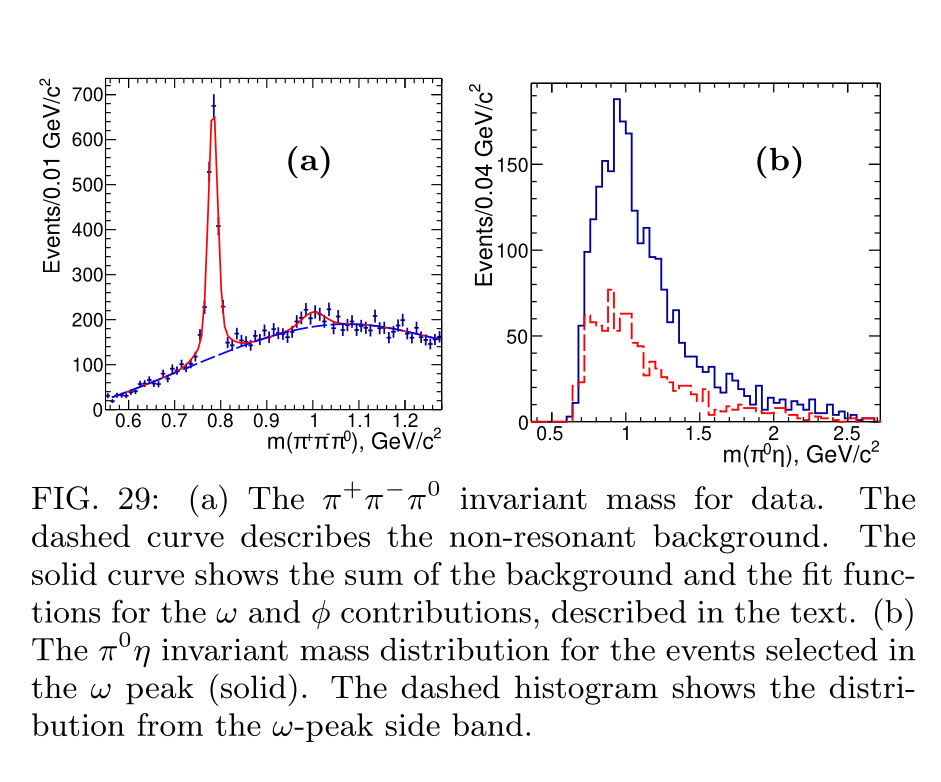
\includegraphics[width=.48\textwidth]{figures/003/fig029}
  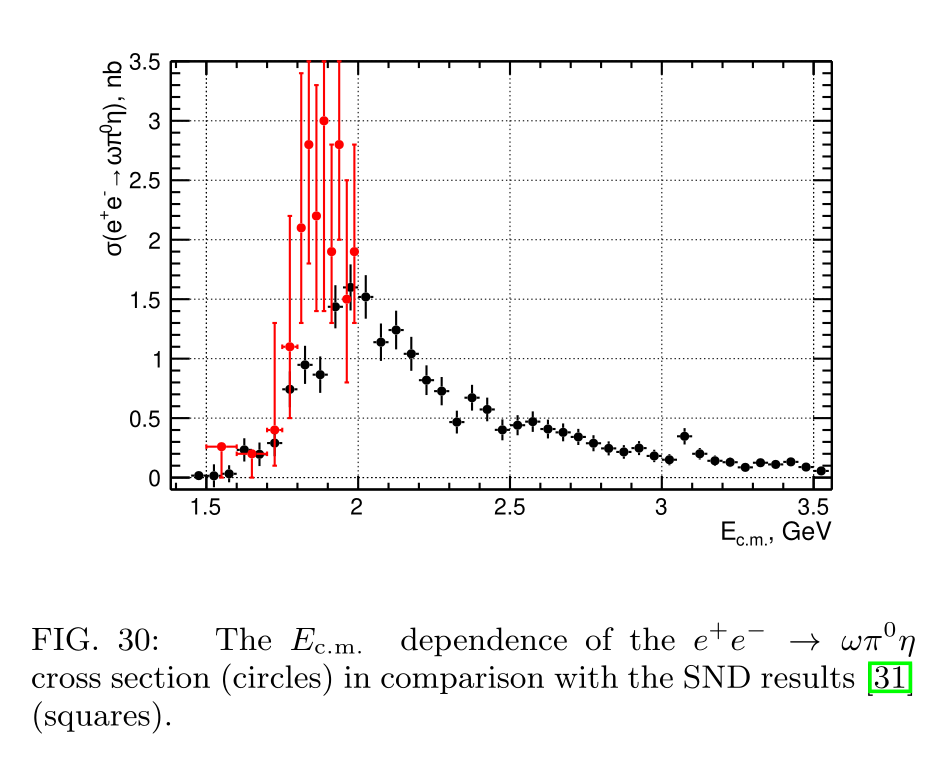
\includegraphics[width=.48\textwidth]{figures/003/fig030}
\end{frame}%}}}

\begin{frame}[label=2pieta-res-rho]%{{{
  \frametitle{$\pip\pim2\piz\eta$: resonant structure: 
  $\rho^\pm\to\pi^\pm\piz$}
  \centering

  $\rho\to\pi\piz$ peaks, $\rhop\rhom$ correlation again \\[1ex]

  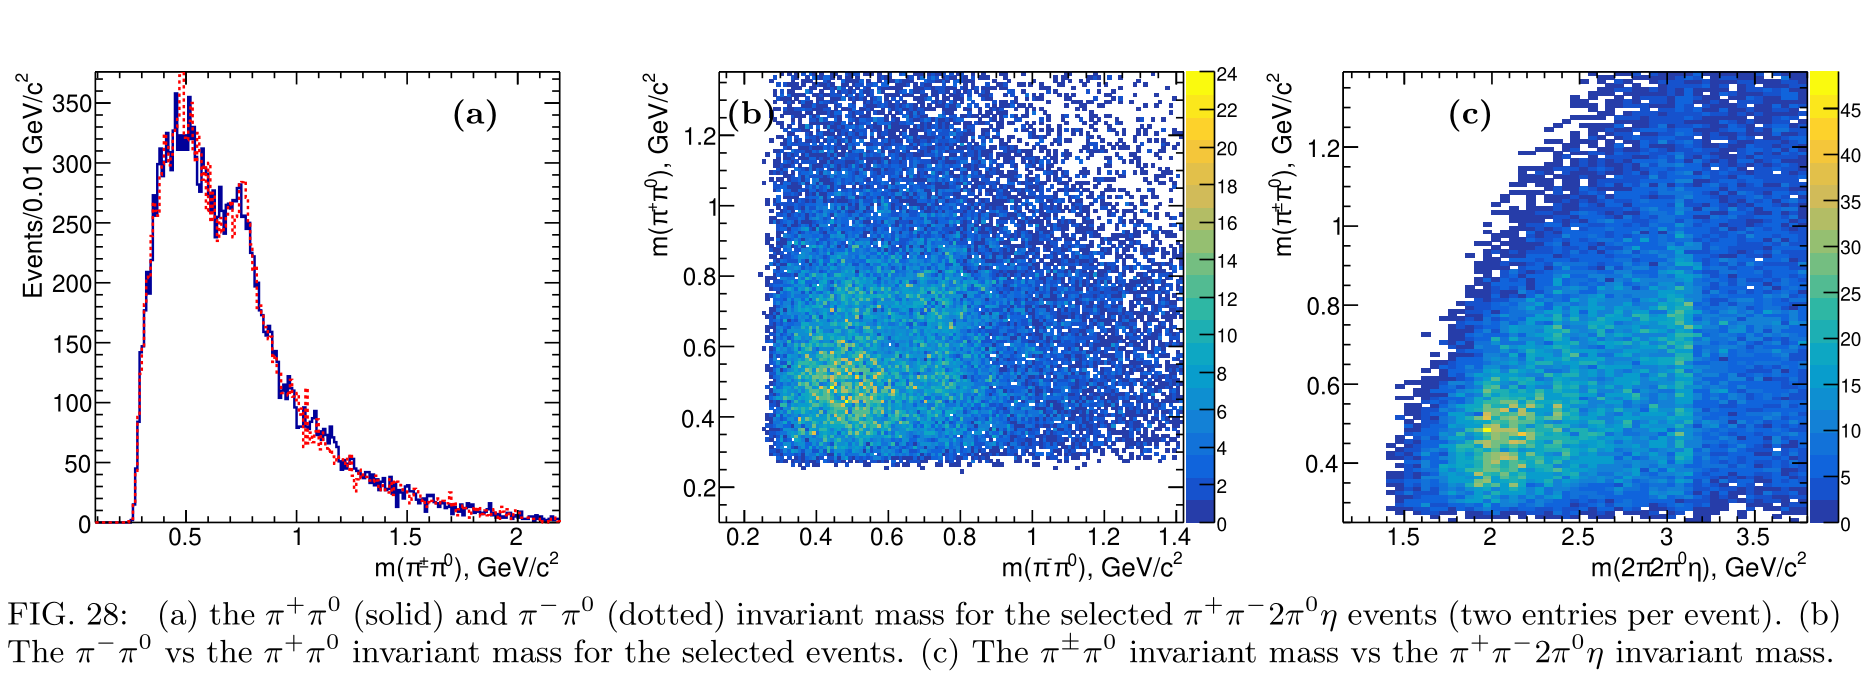
\includegraphics[width=\textwidth]{figures/003/fig028}
\end{frame}%}}}

\begin{frame}[label=2pieta-res-rho]%{{{
  \frametitle{$\pip\pim2\piz\eta$: resonant structure: 
  $\rho^\pm\to\pi^\pm\piz$}
  \centering

  $2908 \pm 202$ events, intermediate $a_0(980)\rho\pi$ is present \\
  Sum of intermediate states is equal to the full cross-section except 
  in the region around 2 GeV \\[1ex]

  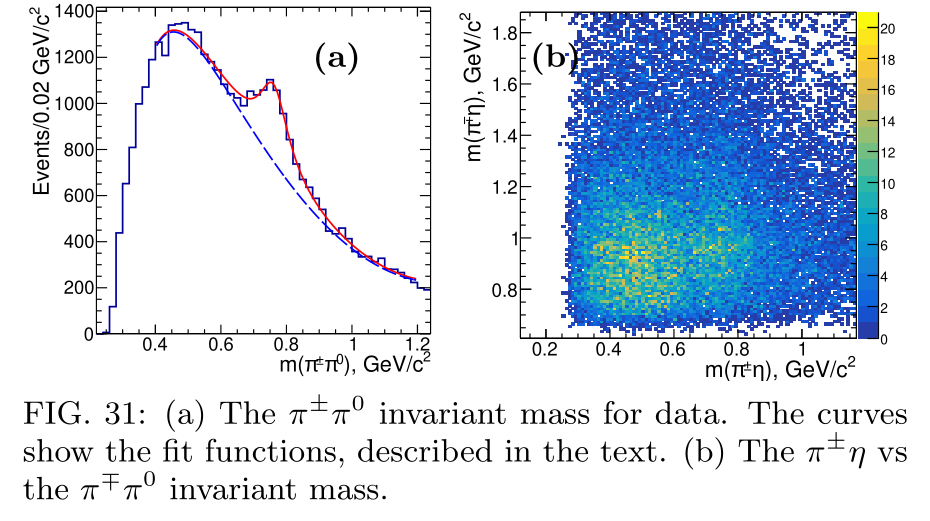
\includegraphics[width=.55\textwidth]{figures/003/fig031}
  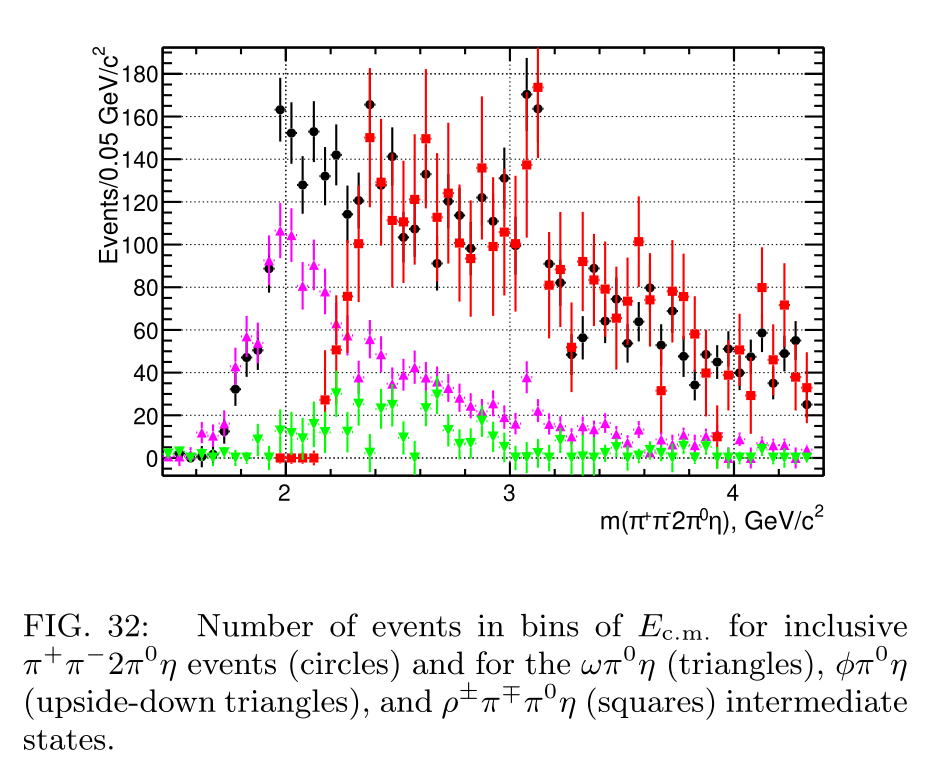
\includegraphics[width=.4\textwidth]{figures/003/fig032}
\end{frame}%}}}

\begin{frame}[label=Jpsi-3pi]%{{{
  \frametitle{$J/\psi$ region in $m(\pip\pim3\piz)$}
  \centering

  $2389 \pm 63$ events with $J/\psi$ and $177 \pm 27$ with $\psi(2S)$ \\
  including $142 \pm 21$ events of $\psi(2S)\to J/\psi\piz\piz\to5\pi$ 
  \\[1ex]

  \begin{tabular}{cc}
    $B_{J/\psi\to5\pi} = (2.70 \pm 0.07 \pm 0.27)\times 10^{-2}$ &
    $B_{\psi(2S)\to5\pi} = (5.2 \pm 0.8 \pm 0.5)\times 10^{-3}$ \\
  \end{tabular}

  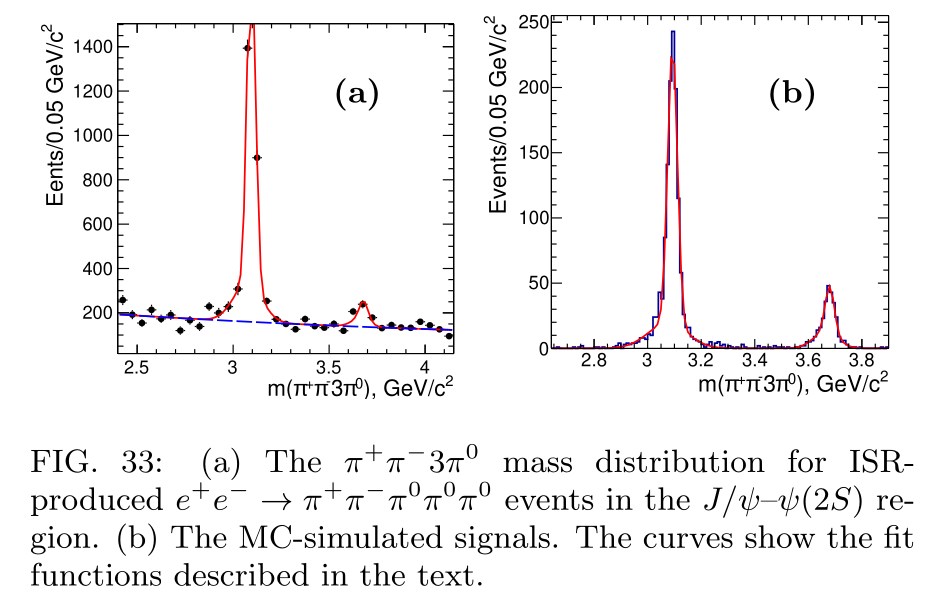
\includegraphics[width=.48\textwidth]{figures/003/fig033}
  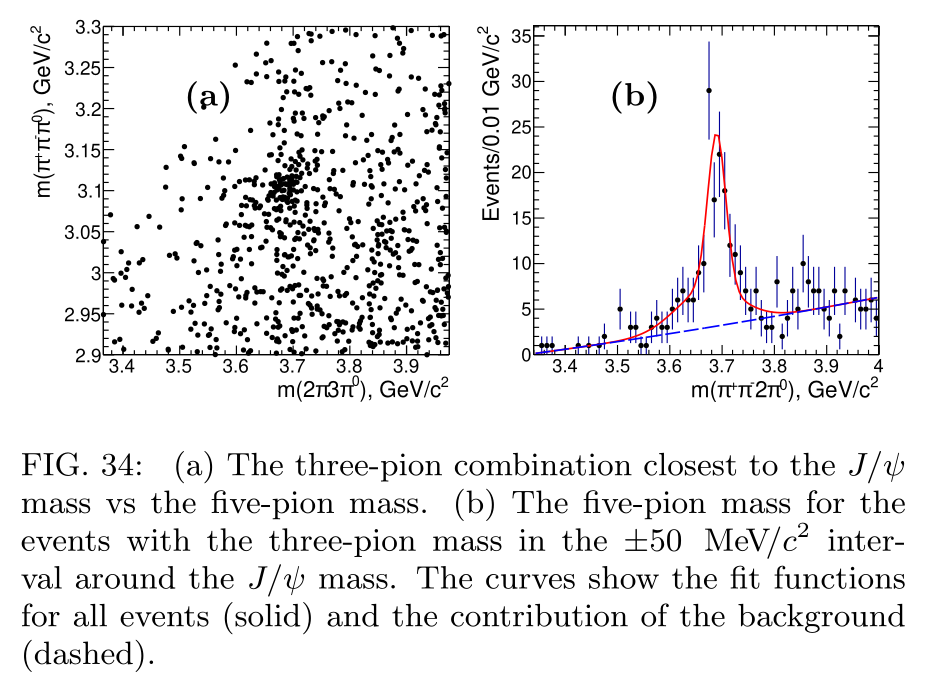
\includegraphics[width=.48\textwidth]{figures/003/fig034}
\end{frame}%}}}

\begin{frame}[label=Jpsi-3pi-intermediate-states]%{{{
  \frametitle{$J/\psi$ region in $m(\pip\pim3\piz)$: intermediate $5\pi$ states}
  \centering

  \begin{tabular}{cc}
    $B_{J/\psi\to\omega\piz\piz} = (5.04 \pm 0.37 \pm 0.50)\times 10^{-3}$ &
    $B_{\psi(2S)\to\omega\piz\piz} = (1.1\pm0.3\pm0.1)\times 10^{-3}$ \\
  \end{tabular}

  $B_{J/\psi\to\omega\piz\piz}$ lower than for $\omega\pip\pim$ by 
  a factor of two, as expected from isospin symmetry, again

  \small
  \begin{tabular}{cc}
    $B_{J/\psi\to\rho^\pm\pi^\mp\piz\piz} = (1.40 \pm 0.12 \pm 0.14 \pm 0.10)\times 10^{-2}$ &
    $B_{J/\psi\to\rhop\rhom\piz} = (0.60 \pm 0.05 \pm 0.06 \pm 0.05)\times 10^{-2}$ \\
  \end{tabular}

  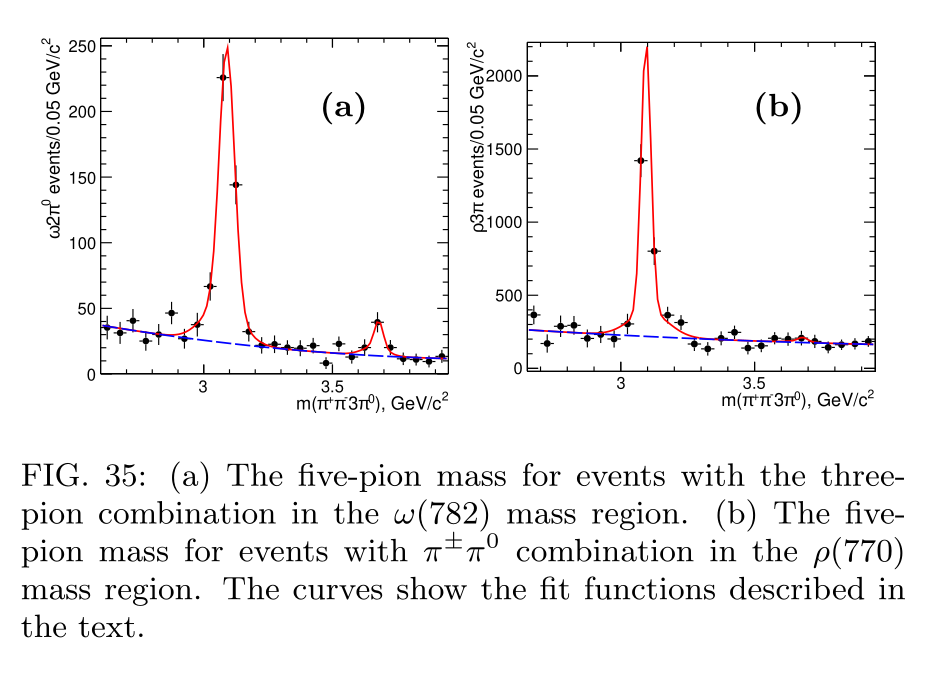
\includegraphics[width=.48\textwidth]{figures/003/fig035}
  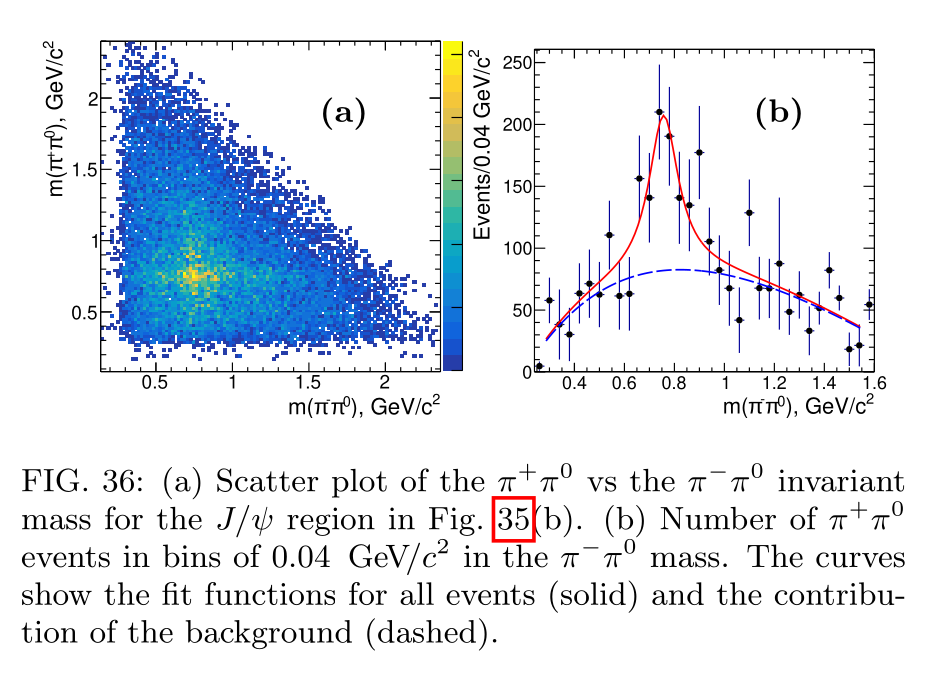
\includegraphics[width=.48\textwidth]{figures/003/fig036}
\end{frame}%}}}

\begin{frame}[label=Jpsi-2pieta]%{{{
  \frametitle{$J/\psi$ region in $m(\pip\pim2\piz\eta)$}
  \centering

  $203\pm29$ $J/\psi\to\pip\pim2\piz\eta$ decays,
  $27\pm14$ $J/\psi\to\omega\piz\eta$ decays,
  $168\pm62$ $J/\psi\to\rho^\pm\pi^\mp\piz\piz$ decays

  \begin{tabular}{cc}
    $B_{J/\psi\to\pip\pim\piz\piz\eta} = (2.30\pm0.33\pm0.35)\times 10^{-3}$ &
    $B_{J/\psi\to\omega\piz\eta} = (3.4\pm1.6\pm0.6)\times 10^{-4}$ \\
    $B_{J/\psi\to\rho^\pm\pi^\mp\piz\eta} = (1.9\pm0.7\pm0.3)\times 10^{-3}$ &
    $B_{\psi(2S)\to\pip\pim\piz\piz\eta} < 3.5 \times 10^{-4}$ at $90\%$ C.L. \\
  \end{tabular}

  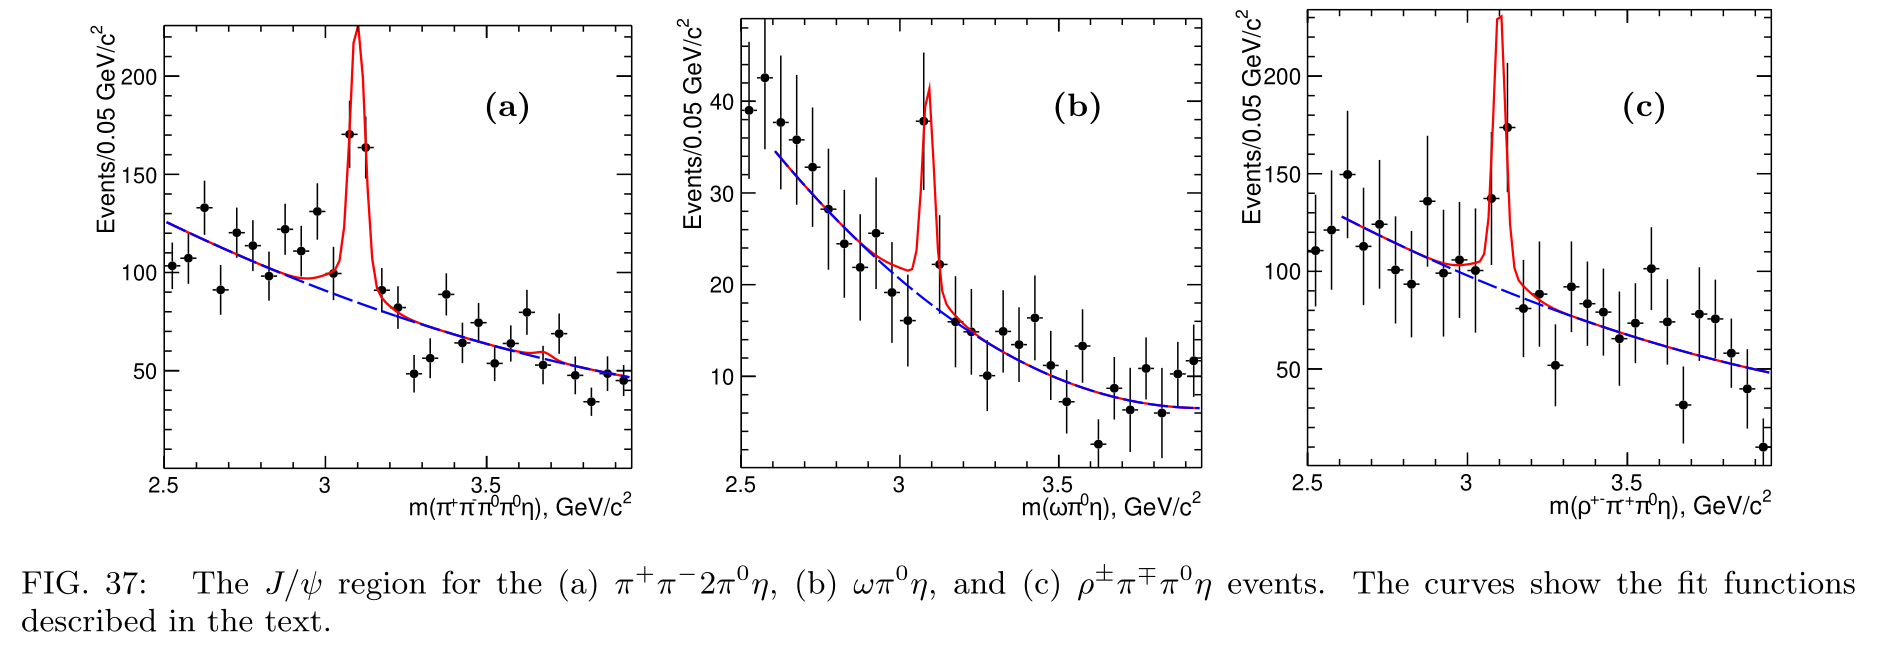
\includegraphics[width=.8\textwidth]{figures/003/fig037}
\end{frame}%}}}

\begin{frame}[label=summary]%{{{
  \frametitle{Summary}
  \large

  \begin{itemize}
    \item Two $ee$ annihilation processes with 5 final state particles 
      were studied at a range center-of-mass energies.
    \item Their cross-sections measured as functions of c.m. energy.
    \item Resonant structure comprehensively investigated including 
      sub-process cross-section measurements.
    \item Branching fractions of several $J/\psi$ and $\psi(2S)$ decay 
      modes measured for the first time.
  \end{itemize}
\end{frame}%}}}

\end{document}
